% Lines starting with a percent sign (%) are comments. LaTeX will 
% not process those lines. Similarly, everything after a percent 
% sign in a line is considered a comment. To produce a percent sign
% in the output, write \% (backslash followed by the percent sign). 
% ==================================================================
% Usage instructions:
% ------------------------------------------------------------------
% The file is heavily commented so that you know what the various
% commands do. Feel free to remove any comments you don't need from
% your own copy. When redistributing the example thesis file, please
% retain all the comments for the benefit of other thesis writers! 
% ==================================================================
% Compilation instructions: 
% ------------------------------------------------------------------
% Use pdflatex to compile! Input images are expected as PDF files.
% Example compilation:
% ------------------------------------------------------------------
% > pdflatex thesis-example.tex
% > bibtex thesis-example
% > pdflatex thesis-example.tex
% > pdflatex thesis-example.tex
% ------------------------------------------------------------------
% You need to run pdflatex multiple times so that all the cross-references
% are fixed. pdflatex will tell you if you need to re-run it (a warning
% will be issued)  
% ------------------------------------------------------------------
% Compilation has been tested to work in ukk.cs.hut.fi and kosh.hut.fi
% - if you have problems of missing .sty -files, then the local LaTeX
% environment does not have all the required packages installed.
% For example, when compiling in vipunen.hut.fi, you get an error that
% tikz.sty is missing - in this case you must either compile somewhere
% else, or you cannot use TikZ graphics in your thesis and must therefore
% remove or comment out the tikz package and all the tikz definitions. 
% ------------------------------------------------------------------

% General information
% ==================================================================
% Package documentation:
% 
% The comments often refer to package documentation. (Almost) all LaTeX
% packages have documentation accompanying them, so you can read the
% package documentation for further information. When a package 'xxx' is
% installed to your local LaTeX environment (the document compiles
% when you have \usepackage{xxx} and LaTeX does not complain), you can 
% find the documentation somewhere in the local LaTeX texmf directory
% hierarchy. In ukk.cs.hut.fi, this is /usr/texlive/2008/texmf-dist,
% and the documentation for the titlesec package (for example) can be 
% found at /usr/texlive/2008/texmf-dist/doc/latex/titlesec/titlesec.pdf.
% Most often the documentation is located as a PDF file in 
% /usr/texlive/2008/texmf-dist/doc/latex/xxx, where xxx is the package name; 
% however, documentation for TikZ is in
% /usr/texlive/2008/texmf-dist/doc/latex/generic/pgf/pgfmanual.pdf
% (this is because TikZ is a front-end for PGF, which is meant to be a 
% generic portable graphics format for LaTeX).
% You can try to look for the package manual using the ``find'' shell
% command in Linux machines; the find databases are up-to-date at least
% in ukk.cs.hut.fi. Just type ``find xxx'', where xxx is the package
% name, and you should find a documentation file.
% Note that in some packages, the documentation is in the DVI file
% format. In this case, you can copy the DVI file to your home directory,
% and convert it to PDF with the dvipdfm command (or you can read the
% DVI file directly with a DVI viewer).
% 
% If you can't find the documentation for a package, just try Googling
% for ``latex packagename''; most often you can get a direct link to the
% package manual in PDF format.
% ------------------------------------------------------------------


% Document class for the thesis is report
% ------------------------------------------------------------------
% You can change this but do so at your own risk - it may break other things.
% Note that the option pdftext is used for pdflatex; there is no
% pdflatex option. 
% ------------------------------------------------------------------
\documentclass[12pt,a4paper,oneside,pdftex]{report}

% Extra package added by me.
% package for writing pseudocode
\usepackage{clrscode3e}
\usepackage{float}


% The input files (tex files) are encoded with the latin-1 encoding 
% (ISO-8859-1 works). Change the latin1-option if you use UTF8 
% (at some point LaTeX did not work with UTF8, but I'm not sure
% what the current situation is) 
\usepackage[latin1]{inputenc}
% OT1 font encoding seems to work better than T1. Check the rendered
% PDF file to see if the fonts are encoded properly as vectors (instead
% of rendered bitmaps). You can do this by zooming very close to any letter 
% - if the letter is shown pixelated, you should change this setting 
% (try commenting out the entire line, for example).  
\usepackage[OT1]{fontenc}
% The babel package provides hyphenating instructions for LaTeX. Give
% the languages you wish to use in your thesis as options to the babel
% package (as shown below). You can remove any language you are not
% going to use.
% Examples of valid language codes: english (or USenglish), british, 
% finnish, swedish; and so on.
\usepackage[finnish,swedish,english]{babel}


% Font selection
% ------------------------------------------------------------------
% The default LaTeX font is a very good font for rendering your 
% thesis. It is a very professional font, which will always be 
% accepted. 
% If you, however, wish to spicen up your thesis, you can try out
% these font variants by uncommenting one of the following lines
% (or by finding another font package). The fonts shown here are 
% all fonts that you could use in your thesis (not too silly). 
% Changing the font causes the layouts to shift a bit; you many
% need to manually adjust some layouts. Check the warning messages
% LaTeX gives you.
% ------------------------------------------------------------------
% To find another font, check out the font catalogue from
% http://www.tug.dk/FontCatalogue/mathfonts.html
% This link points to the list of fonts that support maths, but
% that's a fairly important point for master's theses.
% ------------------------------------------------------------------
% <rant>
% Remember, there is no excuse to use Comic Sans, ever, in any
% situation! (Well, maybe in speech bubbles in comics, but there 
% are better options for those too)
% </rant>

% \usepackage{palatino}
% \usepackage{tgpagella}



% Optional packages
% ------------------------------------------------------------------
% Select those packages that you need for your thesis. You may delete
% or comment the rest.

% Natbib allows you to select the format of the bibliography references.
% The first example uses numbered citations: 
\usepackage[square,sort&compress,numbers]{natbib}
% The second example uses author-year citations.
% If you use author-year citations, change the bibliography style (below); 
% acm style does not work with author-year citations.
% Also, you should use \citet (cite in text) when you wish to refer
% to the author directly (\citet{blaablaa} said blaa blaa), and 
% \citep when you wish to refer similarly than with numbered citations
% (It has been said that blaa blaa~\citep{blaablaa}).
% \usepackage[square]{natbib}

% The alltt package provides an all-teletype environment that acts
% like verbatim but you can use LaTeX commands in it. Uncomment if 
% you want to use this environment. 
% \usepackage{alltt}

% The eurosym package provides a euro symbol. Use with \euro{}
\usepackage{eurosym} 

% Verbatim provides a standard teletype environment that renderes
% the text exactly as written in the tex file. Useful for code
% snippets (although you can also use the listings package to get
% automatic code formatting). 
\usepackage{verbatim}

% The listing package provides automatic code formatting utilities
% so that you can copy-paste code examples and have them rendered
% nicely. See the package documentation for details.
% \usepackage{listings}

% The fancuvrb package provides fancier verbatim environments 
% (you can, for example, put borders around the verbatim text area
% and so on). See package for details.
% \usepackage{fancyvrb}

% Supertabular provides a tabular environment that can span multiple 
% pages. 
%\usepackage{supertabular}
% Longtable provides a tabular environment that can span multiple 
% pages. This is used in the example acronyms file. 
\usepackage{longtable}

% The fancyhdr package allows you to set your the page headers 
% manually, and allows you to add separator lines and so on. 
% Check the package documentation. 
% \usepackage{fancyhdr}

% Subfigure package allows you to use subfigures (i.e. many subfigures
% within one figure environment). These can have different labels and
% they are numbered automatically. Check the package documentation. 
\usepackage{subfigure}

% The titlesec package can be used to alter the look of the titles 
% of sections, chapters, and so on. This example uses the ``medium'' 
% package option which sets the titles to a medium size, making them
% a bit smaller than what is the default. You can fine-tune the 
% title fonts and sizes by using the package options. See the package
% documentation.
\usepackage[medium]{titlesec}

% The TikZ package allows you to create professional technical figures.
% The learning curve is quite steep, but it is definitely worth it if 
% you wish to have really good-looking technical figures. 
\usepackage{tikz}
% You also need to specify which TikZ libraries you use
\usetikzlibrary{positioning}
\usetikzlibrary{calc}
\usetikzlibrary{arrows}
\usetikzlibrary{decorations.pathmorphing,decorations.markings}
\usetikzlibrary{shapes}
\usetikzlibrary{patterns}


% The aalto-thesis package provides typesetting instructions for the
% standard master's thesis parts (abstracts, front page, and so on)
% Load this package second-to-last, just before the hyperref package.
% Options that you can use: 
%   mydraft - renders the thesis in draft mode. 
%             Do not use for the final version. 
%   doublenumbering - [optional] number the first pages of the thesis
%                     with roman numerals (i, ii, iii, ...); and start
%                     arabic numbering (1, 2, 3, ...) only on the 
%                     first page of the first chapter
%   twoinstructors  - changes the title of instructors to plural form
%   twosupervisors  - changes the title of supervisors to plural form
\usepackage[mydraft,twosupervisors]{aalto-thesis}
%\usepackage[mydraft,doublenumbering]{aalto-thesis}
%\usepackage{aalto-thesis}


% Hyperref
% ------------------------------------------------------------------
% Hyperref creates links from URLs, for references, and creates a
% TOC in the PDF file.
% This package must be the last one you include, because it has
% compatibility issues with many other packages and it fixes
% those issues when it is loaded.   
\RequirePackage[pdftex]{hyperref}
% Setup hyperref so that links are clickable but do not look 
% different
\hypersetup{colorlinks=false,raiselinks=false,breaklinks=true}
\hypersetup{pdfborder={0 0 0}}
\hypersetup{bookmarksnumbered=true}
% The following line suggests the PDF reader that it should show the 
% first level of bookmarks opened in the hierarchical bookmark view. 
\hypersetup{bookmarksopen=true,bookmarksopenlevel=1}
% Hyperref can also set up the PDF metadata fields. These are
% set a bit later on, after the thesis setup.   


% Thesis setup
% ==================================================================
% Change these to fit your own thesis.
% \COMMAND always refers to the English version;
% \FCOMMAND refers to the Finnish version; and
% \SCOMMAND refers to the Swedish version.
% You may comment/remove those language variants that you do not use
% (but then you must not include the abstracts for that language)
% ------------------------------------------------------------------
% If you do not find the command for a text that is shown in the cover page or
% in the abstract texts, check the aalto-thesis.sty file and locate the text
% from there. 
% All the texts are configured in language-specific blocks (lots of commands
% that look like this: \renewcommand{\ATCITY}{Espoo}.
% You can just fix the texts there. Just remember to check all the language
% variants you use (they are all there in the same place). 
% ------------------------------------------------------------------
\newcommand{\TITLE}{Software Processes for Dummies:}
\newcommand{\FTITLE}{Ohjelmistoprosessit m�nteille:}
\newcommand{\STITLE}{Den stora stygga vargen:}
\newcommand{\SUBTITLE}{Re-inventing the Wheel}
\newcommand{\FSUBTITLE}{Uusi organisaatio, uudet py�r�t}
\newcommand{\SSUBTITLE}{Lilla Vargens universum}
\newcommand{\DATE}{June 18, 2011}
\newcommand{\FDATE}{18. kes�kuuta 2011}
\newcommand{\SDATE}{Den 18 Juni 2011}

% Supervisors and instructors
% ------------------------------------------------------------------
% If you have two supervisors, write both names here, separate them with a 
% double-backslash (see below for an example)
% Also remember to add the package option ``twosupervisors'' or
% ``twoinstructors'' to the aalto-thesis package so that the titles are in
% plural.
% Example of one supervisor:
%\newcommand{\SUPERVISOR}{Professor Antti Yl�-J��ski}
%\newcommand{\FSUPERVISOR}{Professori Antti Yl�-J��ski}
%\newcommand{\SSUPERVISOR}{Professor Antti Yl�-J��ski}
% Example of twosupervisors:
\newcommand{\SUPERVISOR}{Professor Antti Yl�-J��ski\\
  Professor Pekka Perustieteilij�}
\newcommand{\FSUPERVISOR}{Professori Antti Yl�-J��ski\\
  Professori Pekka Perustieteilij�}
\newcommand{\SSUPERVISOR}{Professor Antti Yl�-J��ski\\
  Professor Pekka Perustieteilij�}

% If you have only one instructor, just write one name here
\newcommand{\INSTRUCTOR}{Olli Ohjaaja M.Sc. (Tech.)}
\newcommand{\FINSTRUCTOR}{Diplomi-insin��ri Olli Ohjaaja}
\newcommand{\SINSTRUCTOR}{Diplomingenj�r Olli Ohjaaja}
% If you have two instructors, separate them with \\ to create linefeeds
% \newcommand{\INSTRUCTOR}{Olli Ohjaaja M.Sc. (Tech.)\\
%  Elli Opas M.Sc. (Tech)}
%\newcommand{\FINSTRUCTOR}{Diplomi-insin��ri Olli Ohjaaja\\
%  Diplomi-insin��ri Elli Opas}
%\newcommand{\SINSTRUCTOR}{Diplomingenj�r Olli Ohjaaja\\
%  Diplomingenj�r Elli Opas}

% If you have two supervisors, it is common to write the schools
% of the supervisors in the cover page. If the following command is defined,
% then the supervisor names shown here are printed in the cover page. Otherwise,
% the supervisor names defined above are used.
\newcommand{\COVERSUPERVISOR}{Professor Antti Yl�-J��ski, Aalto University\\
  Professor Pekka Perustieteilij�, University of Helsinki}

% The same option is for the instructors, if you have multiple instructors.
% \newcommand{\COVERINSTRUCTOR}{Olli Ohjaaja M.Sc. (Tech.), Aalto University\\
%  Elli Opas M.Sc. (Tech), Aalto SCI}


% Other stuff
% ------------------------------------------------------------------
\newcommand{\PROFESSORSHIP}{Data Communication Software}
\newcommand{\FPROFESSORSHIP}{Tietoliikenneohjelmistot}
\newcommand{\SPROFESSORSHIP}{Datakommunikationsprogram}
% Professorship code is the same in all languages
\newcommand{\PROFCODE}{T-110}
\newcommand{\KEYWORDS}{ocean, sea, marine, ocean mammal, marine mammal, whales,
cetaceans, dolphins, porpoises}
\newcommand{\FKEYWORDS}{AEL, aineistot, aitta, akustiikka, Alankomaat,
aluerakentaminen, Anttolanhovi, Arcada, ArchiCad, arkki}
\newcommand{\SKEYWORDS}{oms�ttning, kassafl�de, v�rdepappersmarknadslagen,
yrkesut�vare, intressef�retag, verifieringskedja}
\newcommand{\LANGUAGE}{English}
\newcommand{\FLANGUAGE}{Englanti}
\newcommand{\SLANGUAGE}{Engelska}

% Author is the same for all languages
\newcommand{\AUTHOR}{Stella Student}


% Currently the English versions are used for the PDF file metadata
% Set the PDF title
\hypersetup{pdftitle={\TITLE\ \SUBTITLE}}
% Set the PDF author
\hypersetup{pdfauthor={\AUTHOR}}
% Set the PDF keywords
\hypersetup{pdfkeywords={\KEYWORDS}}
% Set the PDF subject
\hypersetup{pdfsubject={Master's Thesis}}


% Layout settings
% ------------------------------------------------------------------

% When you write in English, you should use the standard LaTeX 
% paragraph formatting: paragraphs are indented, and there is no 
% space between paragraphs.
% When writing in Finnish, we often use no indentation in the
% beginning of the paragraph, and there is some space between the 
% paragraphs. 

% If you write your thesis Finnish, uncomment these lines; if 
% you write in English, leave these lines commented! 
% \setlength{\parindent}{0pt}
% \setlength{\parskip}{1ex}

% Use this to control how much space there is between each line of text.
% 1 is normal (no extra space), 1.3 is about one-half more space, and
% 1.6 is about double line spacing.  
% \linespread{1} % This is the default
% \linespread{1.3}

% Bibliography style
% acm style gives you a basic reference style. It works only with numbered
% references.
\bibliographystyle{acm}
% Plainnat is a plain style that works with both numbered and name citations.
% \bibliographystyle{plainnat}


% Extra hyphenation settings
% ------------------------------------------------------------------
% You can list here all the files that are not hyphenated correctly.
% You can provide many \hyphenation commands and/or separate each word
% with a space inside a single command. Put hyphens in the places where
% a word can be hyphenated.
% Note that (by default) LaTeX will not hyphenate words that already
% have a hyphen in them (for example, if you write ``structure-modification 
% operation'', the word structure-modification will never be hyphenated).
% You need a special package to hyphenate those words.
\hyphenation{di-gi-taa-li-sta yksi-suun-tai-sta}



% The preamble ends here, and the document begins. 
% Place all formatting commands and such before this line.
% ------------------------------------------------------------------
\begin{document}
% This command adds a PDF bookmark to the cover page. You may leave
% it out if you don't like it...
\pdfbookmark[0]{Cover page}{bookmark.0.cover}
% This command is defined in aalto-thesis.sty. It controls the page 
% numbering based on whether the doublenumbering option is specified
\startcoverpage

% Cover page
% ------------------------------------------------------------------
% Options: finnish, english, and swedish
% These control in which language the cover-page information is shown
\coverpage{english}


% Abstracts
% ------------------------------------------------------------------
% Include an abstract in the language that the thesis is written in,
% and if your native language is Finnish or Swedish, one in that language.

% Abstract in English
% ------------------------------------------------------------------
\thesisabstract{english}{
A dissertation or thesis is a document submitted in support of candidature
for a degree or professional qualification presenting the author's research and
findings. In some countries/universities, the word thesis or a cognate is used
as part of a bachelor's or master's course, while dissertation is normally
applied to a doctorate, whilst, in others, the reverse is true.

\fixme{Abstract text goes here (and this is an example how to use fixme).} 
Fixme is a command that helps you identify parts of your thesis that still
require some work. When compiled in the custom \texttt{mydraft} mode, text
parts tagged with fixmes are shown in bold and with fixme tags around them. When
compiled in normal mode, the fixme-tagged text is shown normally (without
special formatting). The draft mode also causes the ``Draft'' text to appear on
the front page, alongside with the document compilation date. The custom
\texttt{mydraft} mode is selected by the \texttt{mydraft} option given for the
package \texttt{aalto-thesis}, near the top of the \texttt{thesis-example.tex}
file.

The thesis example file (\texttt{thesis-example.tex}), all the chapter content
files (\texttt{1introduction.tex} and so on), and the Aalto style file
(\texttt{aalto-thesis.sty}) are commented with explanations on how the Aalto
thesis works. The files also contain some examples on how to customize various
details of the thesis layout, and of course the example text works as an
example in itself. Please read the comments and the example text; that should
get you well on your way!}


% Acknowledgements
% ------------------------------------------------------------------
% Select the language you use in your acknowledgements
\selectlanguage{english}

% Uncomment this line if you wish acknoledgements to appear in the 
% table of contents
%\addcontentsline{toc}{chapter}{Acknowledgements}

% The star means that the chapter isn't numbered and does not 
% show up in the TOC
\chapter*{Acknowledgements}

I wish to thank all students who use \LaTeX\ for formatting their theses,
because theses formatted with \LaTeX\ are just so nice.

Thank you, and keep up the good work!
\vskip 10mm

\noindent Espoo, \DATE
\vskip 5mm
\noindent\AUTHOR

% Acronyms
% ------------------------------------------------------------------
% Use \cleardoublepage so that IF two-sided printing is used 
% (which is not often for masters theses), then the pages will still
% start correctly on the right-hand side.
\cleardoublepage
% Example acronyms are placed in a separate file, acronyms.tex
\addcontentsline{toc}{chapter}{Abbreviations and Acronyms}
\chapter*{Abbreviations and Acronyms}

% The longtable environment should break the table properly to multiple pages, 
% if needed

\noindent
\begin{longtable}{@{}p{0.25\textwidth}p{0.7\textwidth}@{}}
2k/4k/8k mode & COFDM operation modes \\
3GPP & 3rd Generation Partnership Project \\ 
ESP & Encapsulating Security Payload; An IPsec security protocol \\ 
FLUTE  & The File Delivery over Unidirectional Transport protocol \\ 
e.g.& for example (do not list here this kind of common acronymbs or abbreviations, but only those that are essential for understanding the content of your thesis. \\ 
note & Note also, that this list is not compulsory, and should be omitted if you have only few abbreviations

\end{longtable}


% Table of contents
% ------------------------------------------------------------------
\cleardoublepage
% This command adds a PDF bookmark that links to the contents.
% You can use \addcontentsline{} as well, but that also adds contents
% entry to the table of contents, which is kind of redundant.
% The text ``Contents'' is shown in the PDF bookmark. 
\pdfbookmark[0]{Contents}{bookmark.0.contents}
\tableofcontents

% List of tables
% ------------------------------------------------------------------
% You only need a list of tables for your thesis if you have very 
% many tables. If you do, uncomment the following two lines.
% \cleardoublepage
% \listoftables

% Table of figures
% ------------------------------------------------------------------
% You only need a list of figures for your thesis if you have very 
% many figures. If you do, uncomment the following two lines.
% \cleardoublepage
% \listoffigures

% The following label is used for counting the prelude pages
\label{pages-prelude}
\cleardoublepage

%%%%%%%%%%%%%%%%% The main content starts here %%%%%%%%%%%%%%%%%%%%%
% ------------------------------------------------------------------
% This command is defined in aalto-thesis.sty. It controls the page 
% numbering based on whether the doublenumbering option is specified
\startfirstchapter

% Add headings to pages (the chapter title is shown)
\pagestyle{headings}

% The contents of the thesis are separated to their own files.
% Edit the content in these files, rename them as necessary.
% ------------------------------------------------------------------
\chapter{Introduction}
\label{chapter:intro}

This is my master's thesis, and I am very proud of it.  Of course,
when I write my \emph{real} master's thesis, I will not use the
singular pronoun \emph{I}, but rather try to avoid referring to myself
and speak of the research \emph{we} have conducted---I rarely work
alone, after all.  Yet, both \emph{I} and \emph{we} are correct, and
it depends on the instructor and the supervisor (of course from you,
too), which one they would prefer. Anyway, the tense should be active,
and passive sentenses should be avoided (especially, writing sentences
where the subject is presented with by preposition), so often you
cannot avoid choosing between the pronouns. Life is strange, but there
you have it.

By the way, the preferred order of writing your master's thesis is
about the same as the outline of the thesis: you first discover your
problem and write about that, then you find out what methods you
should use and write about that.  Then you do your implementation, and
document that, and so on.  However, the abstract and introduction are
often easiest to write last.  This is because these really cover the
entire thesis, and there is no way you could know what to put in your
abstract before you have actually done your implementation and
evaluation. Rarely anyone write the thesis from the beginning to the
end just one time, but the writing is more like process, where every
piece of text is written at least twice. Be also prepared to delete
your own text. In the first phase, you can hide it into comments that
are started with \% but during the writing, the many comments should be
visible for your helpers, the instructor and supervisor.

The introduction in itself is rarely very long; two to five pages often
suffice.


\section{Problem statement}

Undergraduate students studying technical subjects do not consider typography
very interesting these days, and therefore the typographical quality of many
theses is unacceptably low. 
We plan to rectify this situation somewhat by providing a decent-quality
example thesis outline for students.
We expect that the typographical quality of the master's theses will
dramatically increase as the new thesis outline is taken into use.

\section{Helpful hints}

Read the information from the university master's thesis
pages~\cite{ThesisInstructions} before starting the thesis.  You
should also go through the thesis grading
instructions~\cite{ThesisGrading} together with your instructor and/or
supervisor in the beginning of your work.

\section{Structure of the Thesis}
\label{section:structure} 

You should use transition in your text, meaning that you should help
the reader follow the thesis outline. Here, you tell what will be in
each chapter of your thesis. 



\chapter{Background}
\label{chapter:background} 

The problem must have some background, otherwise it is not
interesting.  You can explain the background here. Probably you should
change the title to something that describes more the content of this
chapter. Background consists of information that help other masters of
the same degree program to understand the rest of the thesis.

Transitions mentioned in Section~\ref{section:structure} are used also
in the chapters and sections. For example, next in this chapter we
tell how to use English language, how to find and refer to sources,
and enlight different ways to include graphics in the thesis.

\section{Language and Structure}

Moreover, the transitions are also used in the paragraph and the
sentence level meaning that all the text is linked together. For example,
the word ``moreover'' here is one way, but of course you should use
variation in the text. Examples of transitional devices (words) and
their use can be found from writing guides, e.g. from the Online
Writing Lab
(OWL)\footnote{http://owl.english.purdue.edu/owl/resource/574/02/} of
Purdue University or Strunk's Elements of
Style\footnote{http://www.bartleby.com/141/}. Remember that footnotes
are additional information, and they are seldom used.  If you refer to a source, you do no
not use footnote. The right command for the references is \emph{cite}.

The language used in the thesis should be technical (or
scientifical). For example, the abreviations aren't used but all them
are written open (i.e. ``are not''). Since the content itself is often
hard to understand (and explain), the sentences should not be very
long, use complex language with several examples embedded in the same
sentence, and, also, seldom used words and weird euphemism or paraphrases
can make the sentence hard to follow and to read it with only one
time, and making everything even harder to understand all this without
any punctuation marks makes the instructor cry and finally after
trying to correct the language, you will get boomerang, and everyone's
time has just been wasted.

Please use proofreaders before sending even your unfinished version to
the instructor and/or supervisor. You will get better comments when
they do not need first proofread your text. Moreover, they can
consentrate to the content better if the language and spelling
mistakes are not distracting the reading. Several editors have their
own proofreading tools, e.g. ispell in emacs. You can also use
Microsoft Word to proofread your thesis: it can correct also some
grammatical errors and not just misspelled words.

Note also that if you have a section or a subsection, you have to have
at least two of them, or otherwise the section or subsection title is
unnecessary. Same with the paragraphs an: you should not have sections
with only one paragraphe, and single sentence paragraph. Furthermore,
always write some text after the title before the next level title.

\section{Finding and referring to sources}

Never ever copy anything into your theses from somebody else's text
(nor your own previously published text). Never. Not even for starting
point to be rewritten later. The risk is that you forgot the copied
text to your thesis and end up to be accused of plagiarism. Plagiarism
is a serious crime in studies and science and can ruin your career
even its beginning. To repeate: never cut and paste text into your
thesis!

\subsection{Finding sources}

All work is based on someone else's work. You should find the relevant
sources of your field and choose the best of them. Also, you should
refer to the original source where a fact has been mentioned first
time. Remember source evaluation (criticism) with all sources you
find.

Good starting points for finding references in computer science are: 
\begin{itemize}
% You can use this command to set the items in the list closer to each other
% (ITEM SEParation, the vertical space between the list items) 
\setlength{\itemsep}{0pt}
\item Nelli Portal (Aalto Library): \url{http://www.nelliportaali.fi}
\item ACM Digital library: \url{http://portal.acm.org/}
\item IEEExplore: \url{http://ieeexplore.ieee.org}
\item ScienceDirect: \url{http://www.sciencedirect.com/}
\item \ldots although Google Scholar (\url{http://scholar.google.com/}) will
find links to most of the articles from the abovementioned sources, if you
search from within the university network
\end{itemize}

Some of the publishers do not offer all the text of the articles
freely, but the library has agreed on the rights to use the whole
text. Thus, you should sometimes use computers in the domain of the
university in order to get the full text. Sometimes the Nelli Portal
can also help getting the whole article instead of just the abstract.
The library has also brief instrucions how to find
information~\cite{howfindinfo}.

Instead of normal Google, use Google Scholar
(\url{http://scholar.google.fi/}). It finds academic publications whereas
normal Google find too much commercial advertisements or otherwise
biased information. Wikipedia articles should be referred to in the master
thesis only very, very seldomly. You can use Wikipedia for understanding
some basics and finding more sources, but often you cannot be sure if
the article is correct and unbiased.

One important part of the sources that you have found is the reference
list. This way you can find the original sources that all the other
research of the field refer. Often you can also find more information
with the name of the researchers that are often referred in the
articles.

\subsection{Referring to sources}

The main point in referring to sources is to separate your own
thinking and text from that of others. Facts of the research area can
be given without reference, but otherwise you should refer to
sources. This means two things: marking the source in the text where
it has been used, and listing the sources usually in the end of the
thesis in a way that help the reader to find the original source.

There are several bibliography styles, meaning how to form the
bibliography in the end of the thesis. Aalto's library has good
instructions for many styles~\cite{bibinstructions}. You should ask
from your supervisor or instructors which style you should use. This
thesis template uses the number style that is often used in software
engineering. The other style also used in the CS field,
e.g. usability, is the Harvard style where instead of numbers, the
reference is marked into the text with author's name and publishing
year. Other areas use also many other styles for making the lists and
marking the references.

In addition to the list in the end of the thesis, you have to mark the
source in the text where the source is used. There are three places
for the reference: in a sentence before the period, in the end of a
sentence after the period, or in the end of a paragraph. All of them
have different meaning. The main point is that first you paraphrase
the source using your own words and then mark the source. Next, we
give short examples that are marked with \emph{emphasised text}.

\emph{Haapasalo~\cite{HaapasaloThesis} researched database algorithms
  that allows use of previous versions of the content stored in the
  database.} This kind of marking means that this paragraph (or until
the next reference is given) is based on the source mentioned in the
beginning.  Giving the source you should use only the family name of
the first author of the article, and not give any hints about what is
the type of the article that is referred.

\emph{B+-trees offers one way to index data that is stored in to a
  database. Multiversion B+-trees (MVBT) offer also a way to restore
  the data from previous versions of the database. Concurrent MVBT
  allows many simultaneous updates to the database that is was not
  possible with MVBT.~\cite{HaapasaloThesis}} When the marking is
after the period, the reference is retrospective: all the paragraph
(or after previous reference marking) is based on the source given in
its end. If the content is very broad, you can start with saying
\emph{According to Haapasalo}, then continue referring the source with
several separate sentences, and in the end put the marking of your
source \emph{ that shows that CMVBT are the
  best. ~\cite{HaapasaloThesis}}. 

If your paragraph has several sources, the above mentioned styles are
not proper. The reader of your thesis cannot know which of your
sources give which of the statements. In this case, it is better to
use more finegraded refering where the reference markings that are
embedded in the sentences. For example, \emph{the multiversion B+-tree
  (MVBT) index of Becker et al.~\cite{becker:1996:mvbt} allows database
  users to query old versions of the database, but the index is not
  transactional.
  It's successor, the transactional MBVT (TMVBT), allows a single transaction
  running in its own thread or process to update the database concurrently
  with other transactions that only read the
  database~\cite{haapasalo:2009:tmvbt}. 
  Further development, titled the concurrent MBVT (CMVBT),
  allows several transactions to perform updates to the database at the same
  time~\cite{HaapasaloThesis}}. 
  Here, the references are marked before
  the period in the sentences where they are used.

Finally, direct quotes are allowed. However, often you should avoid
them since they do not usually fit in to your text very well. Using
direct quotes has two tricks: quotation marks and the source.  \emph{
  ``Even though deletions in a multiversion index must not physically
  delete the history of the data items, queries and range scans can
  become more efficient, if the leaf pages of the index structure are
  merged to retain optimality.''~\cite{HaapasaloThesis}} Quotes are
hard to make neatly since you should use only as much as needed
without changing the text. Moreover, you often do not really
understand what the author has mentioned with his wordings if you
cannot write the same with your own words. Remember also that never
cut and paste anything without marking the quotation marks right away,
and in general, never cut and paste anything at all!

Sometimes getting the original source can be almost impossible. In an
extremely desperate situation, you can refer with structure \emph{mr
  X~[\ldots] according to ms Y~[\ldots] defined that}, if you find a
source that refers to the original source. Note also that the
reference marking is never used as sentence element (example of how 
\textbf{not} to do it: \emph{\cite{HaapasaloThesis} describes
an optimal algorithm for indexing multiversiond databases.}).



\chapter{Clustering Patient Visits}
\label{chapter:clustering}

As described in Chapter XX, all patients data is retrieved from the database directly without any manual labeling. Due to lack of labels, unsupervised learning algorithms should be adopted. Clustering is a collection of unsupervised methods, which identifies groups of data points according to a defined similarity metric, such that objects in the same group posses higher similarities compared to objects in other groups. The clustering process does not rely on labels but the choice of similarity metrics. Variations in similarity metrics lead to different clustering methods.

Applying clustering methods in anomaly detection tasks has been studied numerously~\cite{he2003discovering}
. This chapter introduces two typical methods, K-Means~\cite{lloyd1982least} and DBSCAN~\cite{ester1996density}. Problem formulation, solutions, and potential issues are formally described using elaborated notations in following sections. However, analysis on the performance and constraints of these two methods are postponed to Chapter XXX, which reveals their practicality and infeasibility in the previously described anomaly detection problem. (Time, Memory consumption. For K-Means, definition of center.)

\section{K-Means}
\label{sec:k-means}

K-Means is one of the simplest unsupervised algorithm which solves clustering problem. Despite its simplicity, K-Means has gained success in various situations, including anomaly detection~\cite{he2003discovering}~\cite{campello2015hierarchical}, image segmentation and compression~\cite{forsyth2002computer}, and preprocessing for more complicated algorithms. The method can be formally defined as follow: Given a data set $\{\mathbf{x}_1, ... , \mathbf{x}_N\}$ consisting of $N$ observations in $D$-dimensional space, the object is to partition the data into $K$ groups, by defining a set of $K$ centers $\{\boldsymbol{\mu}_1, ... , \boldsymbol{\mu}_k\}$ in the same space, and assigning each observation to exactly one center point. Each center point represents a prototype associated with the $k^{th}$ cluster.

The assignments can be represented using 1-of-$K$ scheme. Then, for each data point $x_n$, a corresponding  $K$-dimensional variable consisting of $K$ binary elements $r_{nk} \in \{0, 1\}$ is introduced. Among these $r_{nk}$, exactly one of them equals 1, which means $\mathbf{x}_{n}$ belongs to the $k^{th}$ cluster. Using this notation, evaluation of the clustering quality can be defined using the object function as follow:
\begin{equation}	
	\label{eq:kmeansobj}
	J = \sum_{n=1}^{N}\sum_{k=1}^{K}r_{nk}D(\mathbf{x}_{N} - \boldsymbol{\mu}_{k})
\end{equation}
where $D$ is the dissimilarity metric. Common choice of the metric is $\mathit{l}_1$-norm or $\mathit{l}_2$-norm. Mahalanobis distance is also adopted while considering the covariances between the $K$-dimensions~\cite{davis1986statistics}. In the following context, $\mathit{l}_2$-norm is adoped for discussion. 
 Intuitively, this function can be considered as the distance summation of each point to its corresponding cluster prototype $\boldsymbol{\mu}_k$. The K-Means aims at finding a set of $\boldsymbol{\mu}_k$ which minimizes the object function. Finding the optimal solution for the above object function proves to be NP-Hard~\cite{aloise2009np}. However, employing heuristic algorithms enables finding converged local optimal solutions. Section~\ref{subsec:EM} describes one iterative algorithm, EM. Section~\ref{subsec:KMeansIssues} explores common issues related to K-Means and remedies.
\subsection{EM Algorithm in K-Means}
\label{subsec:EM}

EM algorithm is an iterative algorithm to find local maximum. Each iteration consists of two phases, Expectation and Maximization, which corresponds to minimize the objective function $J$ with respect to $r_{nk}$ and $\boldsymbol{\mu}_{k}$ respectively. In the E(expectation) step, the algorithm minimize $J$ with respect to $r_{nk}$, while keeping the $\boldsymbol{\mu}_{k}$ fixed. Then in the following M(maximization) step, the algorithm minimizes $J$ with respect to $\boldsymbol{\mu}_{k}$, while keeping $r_{nk}$ fixed. 

Considering the optimization in E step, a critical observation of \eqref{eq:kmeansobj} is that \(\mathbf{r}_n\)'s are independent of each other. Thus, optimization on \(\mathbf{r}_n\)'s can be done seperately for each \(n\). The solution is simply setting the \(r_{nk}\) corresponding to the minimum \(\| \mathbf{x}_n - \boldsymbol{\mu}_k \|^2\) to 1.  Intuitively, the algorithm assigns \(\mathbf{x}_n\) to the closest cluster center. Formally, the solution can be written as
\begin{equation}
 r_{nk} =
    \begin{cases}
        1   & \quad \text{if } k = \operatorname{arg\,min}_j \parallel \mathbf{x}_{n} - \mathbf{\mu}_{j} {\parallel}^2 \\
        0   & \quad \text{otherwise}
    \end{cases}
\end{equation}

In the following M step, the above determined \(r_{nk}\) is clamped. Then, \(\boldsymbol{\mu}_k\) appears only in a quadratic term in \(J\). Setting derivatives of \(J\) with respect to \(\boldsymbol{\mu}_k\) to zero, solution formula for \(\boldsymbol{\mu}_k\) can be expressed in following closed form
\begin{equation}
	\label{eq:muupdate}
	\boldsymbol{\mu}_{k} = \frac{\sum_n r_{nk}\mathbf{x}_n}{\sum_n r_{nk}}
\end{equation}
This step can be considered as recomputing the cluster prototype by setting \(\boldsymbol{\mu}_k\) to the mean of all points assigned to that cluster. 

EM keeps executing these two steps alternatively, until a convergence happens or until number of iterations exceeded a predifined value. Since in each phase, one variable is fixed and updating another variable minimizes the cost function \(J\), convergence is guaranteed. Formal proof on convergence has been studied by MacQueen~\cite{macqueen1967some}.

The algorithm is illustrated using dataset generated independently from three gaussian distributions in Figure~\ref{fig:EM4KMeans}. In this demonstration, the algorithm takes \(K\) = 3, which is the correct number of components. Before running the first iteration, initialized \(\boldsymbol{\mu}_k\) is required. This initialization is done by choosing three objects from the data set randomly.

\begin{figure}
	\begin{center}
		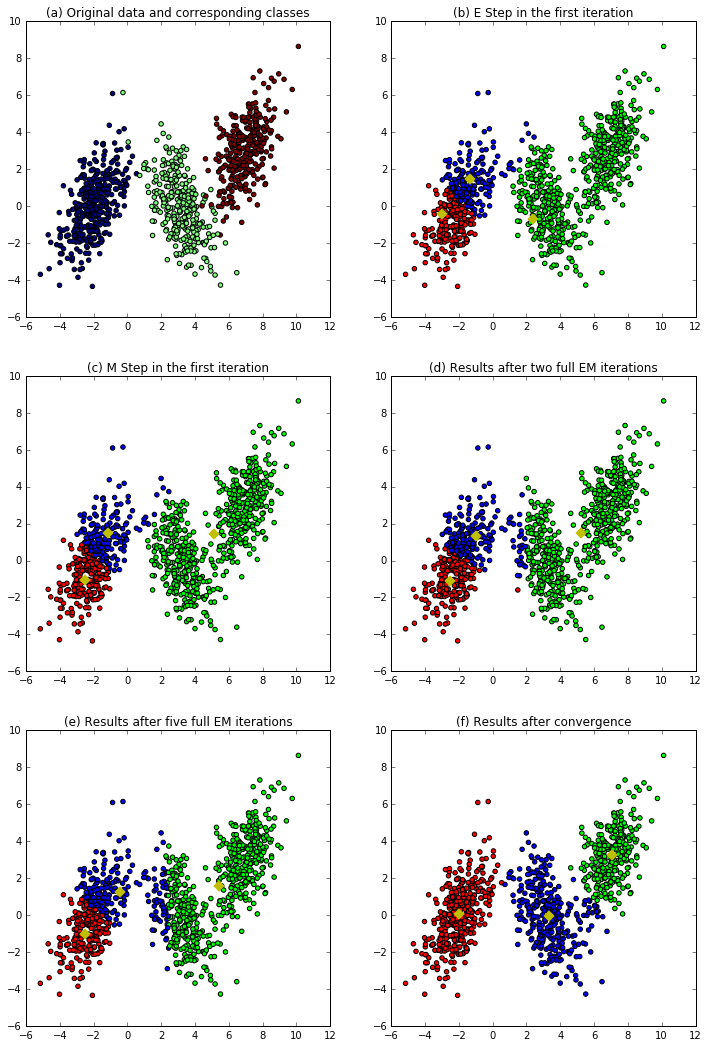
\includegraphics[width=\textwidth]{images/EM4KMeans.png}
		\caption{Illustraion of EM algorithm on K-Means using data generated independently from three gaussian distribution. (a) Original data and corresponding classes. Classes are denoted in different colors. (b) Assignments of each data after the first E step. The yellow diamonds represent the intialized \(\boldsymbol{\mu}_k\). (c) Updated \(\boldsymbol{\mu}_k\) after the M step in the first iteration. (d)-(f) Clustering results after several successive full EM iterations until convergence is met.}
		\label{fig:EM4KMeans}
	\end{center}
\end{figure}

\subsection{Issues in K-Means}
\label{subsec:KMeansIssues}
Despite the simplicity of K-Means, several underlying issues exists. The first potential is that, how to choose the value for \(K\). In the above illustration, \(K\) was set to 3 which is the correct number of components. However, if \(K\) wasn't set to the correct value, unsatisfied clustering may be generated. Example of this issue is shown in Figure~\ref{fig:KMeansIssue}(a)-(c). To solve this problem, one practical way is drawing graph of the cost function versus value of \(K\), as shown in Figure~\ref{fig:KMeansIssue}(d). Intuitively, when \(K\) is under smaller than the true number of clusters, increasing \(K\) will lead to a huge drop of cost function value. However, when \(K\) has reached or exceeded the correct value, incresing \(K\) leads only small cost function value drop. Thus, number of clusters corresponding to the `elbow' point can be considered as the real number of clusters.

\begin{figure}
	\begin{center}
		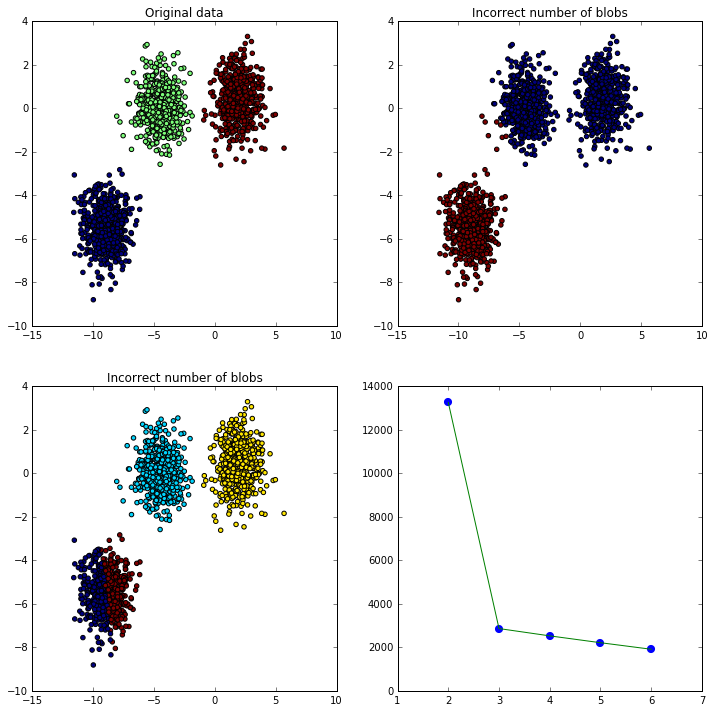
\includegraphics[width=\textwidth]{images/KMeansIncorrectNumber.png}
		\caption{Issues of K-Means incurred by choosing inappropriate value for \(K\)}
		\label{fig:KMeansIssue}
	\end{center}
\end{figure}

Another issues of K-Means relates to the initialization of \(\boldsymbol{\mu}_k\). Since EM finds only local optimal solutions, a poor initialization could lead to worse clustering result. To avoid this problem, it is practical to run K-Means for several times and choose the best result according to the value of the cost function.

One more critical issue of K-Means lies in the choice of similarity metric. As mentioned at the beginning of this chapter, variations in similarity metric leads to different clustering methods. Choosing \(l\)-2 norm is convenient in terms of computation, but this choice limits the type of data variables to certain types. Using \(l\)-2 norm on categorical data is inappropriate since no ordering of categorical values exists. Also, this makes computing the mean value a hard problem. To use K-Means on other data types, the similarity metric should be elaborately designed. 

Besides, K-Means tends to form clusters into a convex space. As shown in Figure~\ref{fig:EM4KMeans}(b)-(e), the boundary between two different clusters forms a line lying at the midway and is perpendicular to the line connecting two cluster prototypes. However, a cluster is not necessary to be convext. This also limits the application of K-Means.

Finally, K-Means is also sensitive to noises. As shown in formula \ref{eq:muupdate}, updating \(\boldsymbol{\mu}_k\) involves computing the mean of all data points assigned to that cluster. When noise objects with large deviation from other points in this cluster exist, update of \(\boldsymbol{\mu}_k\) will be strongly affected. 

\section{Density Based Clustering Methods}
This section explores another type of clustering method which forms cluster from the view of density aspect. \textbf{D}ensity-\textbf{B}ased \textbf{S}patial \textbf{C}lustering of \textbf{A}pplications with \textbf{N}oise (DBSCAN)~\cite{ester1996density} considers to be one of the most successful method from this category~\cite{2014timeaward}. Compared to K-Means, DBSCAN posseses following advantages: 1).\ DBSCAN can detect clusters of arbitrary shape. 2).\ DBSCAN can determine the number of clusters automatically. 3).\ DBSCAN is robust to noises. 

The following of this chapter is organized as follows. Section~\ref{subsec:DBSCANDFS} compares and reveals the relation of DBSCAN to a basic graph traversal algorithm \textbf{D}epth \textbf{F}irst \textbf{S}earch(DFS). This section will introduce the critical concept used by DBSCAN which differentiate it with DFS. Section ~\ref{subsec:DBSCANnotion} describe this concept in more details. Section~\ref{subsec:DBSCANalgorithm} compares DBSCAN and K-Means, and discusses practical issues of DBSCAN.

\subsection{DBSCAN and DFS}
\label{subsec:DBSCANDFS}
Before introducing DBSCAN, it would be helpful to review a basic graph traversal algorithm, DFS, which is an algorithm which traverses or visits a graph. In the discussion of this context, the whole process is divided into two procedures \proc{DFS} and \proc{DFS-Visit}. A typical recursive implementation is described as follow. 

\begin{codebox}
\Procname{$\proc{DFS}(G)$}
\li \For each vertex $u \in G$
\li		\Do
			$\attrib{u}{visited} \gets \const{false}$
	\End
\li	\For each vertex $u \in G$
\li		\Do
		\If \(\attrib{u}{visited} \isequal \const{false}\)
\li			\Then
				$\proc{DFS-Visit}(G, u)$
		\End
	\End
\end{codebox}

\begin{codebox}
\Procname{$\proc{DFS-Visit}(G, u)$}
\li	$\attrib{u}{visited} \gets \const{true}$
\li	\For each vertex $v \in \attrib{G}{Adj}[u]$
\li	\Do
		\If	$\attrib{v}{visited} \isequal \const{false} $
\li			\Then
				$\proc{DFS-Visit}(G, v)$
		\End
	\End
\end{codebox}

The first two lines in \proc{DFS} initializes the algorithm by setting all nodes to be unvisited. Then, the algorithm traverse vertices in the graph. Once an unvisited node is found, \proc{DFS-Visit} is called. In the procedure \proc{DFS-Visit}, the given node $u$ is labled as visited. If an unvisited child $v$ of $u$ is found, this procedure goes one layer deeper by calling another \proc{DFS-Visit} on $v$. After finishing $\proc{DFS-Visit}(G, u)$, the algorithm backtrack to visit other unvisited children of $u$, which are siblings of $v$.

Assume \proc{DFS} executes on an undirected graph. Each call of $\proc{DFS-Visit}$ on an unvisited node $u$ explores $u$ and all nodes reachable to it. These nodes form a component which disconnects with other components by other runs of $\proc{DFS-Visit}$. Thus, each component can be considered as a cluster. The criterion to form a cluster is that each pair of nodes can reache each other through a path consisting of nodes only in this cluster.

DBSCAN can be seen as an application of DFS. However, DBSCAN differs from standard DFS from its useage of \proc{DFS-Visit}. In standard DFS, the algorithm goes deeper by calling $\proc{DFS-Visit}(G, v)$ on all unvisited children of node $u$. In DBSCAN, however, the algorithm goes deeper if and only if node $u$ satisfies extra conditions, which are specified by two user given value $Eps$ and $MinPts$. These extra conditions make the component generated from DBSCAN a meaningful cluster viewing from the density side. The pseudocode is shown below.

\begin{codebox}
\Procname{$\proc{DBSCAN}(S, Eps, MinPts)$}
\li	$\id{ClusterId} \gets 1$
\li	\For each point $u \in S$
\li	\Do
		\If $\attrib{u}{label} \neq \const{nil}$
\li		\Then	
			\kw{continue}
		\End		
\li			$\attrib{u}{neighbor} \gets \proc{Region-Query}(u, Eps)$
\li			\If	$\| \attrib{u}{neighbor} \| < MinPts $
\li				\Then
					$\attrib{u}{label} \gets \const{noise}$
\li			\Else
\li				$\proc{Expand-Cluster}(u, \id{ClusterId}, Eps, MinPts)$
\li				$\id{ClusterId} \gets \id{ClusterId} + 1$
			\End
	\End
\end{codebox}

\begin{codebox}
\Procname{$\proc{Expand-Cluster}(u, \id{ClusterId}, Eps, MinPts)$}
\li	$\attrib{u}{label} \gets \id{ClusterId}$
\li	\For each point $v \in \attrib{u}{neighbor}$
\li	\Do
		\If $\attrib{v}{label} \isequal \const{nil}$
\li		\Then
			$\attrib{v}{label} \gets \id{ClusterId}$
\li			$\attrib{v}{neighbor} \gets \proc{Region-Query}(v, Eps)$
\li				\If	$\| \attrib{v}{neighbor} \| < MinPts $
\li				\Then
					$\proc{Expand-Cluster}(v, \id{ClusterId}, Eps, MinPts)$
				\End
\li		\ElseIf $\attrib{v}{label} \isequal \const{noise}$
\li		\Then
			$\attrib{v}{label} \gets \id{ClusterId}$
		\End
	\End
\end{codebox}

Similiar with DFS traverse, DBSCAN clustering is also divided into two procedures, \proc{DBSCAN} and \proc{Expand-Cluster}. \proc{DBSCAN} functions as a wrapper function in the same way as \proc{DFS}. This procedure goes through each point in the data set $S$. If the current point $u$ has been visited, the procedure skips it. Otherwise, further process continues. However, unlike calling \proc{DFS-Visit} on every unvisited $u$ unconditionaly as \proc{DFS} does, in \proc{DBSCAN}, another procedure \proc{Expand-Cluster} is called if and only if $u$ has sufficient number of neighbors in a given range $Eps$. $\proc{Region-Query}(u, Eps)$ returns all the neighbors of $u$ with a distance no further than $Eps$. This is the extra condition mentioned earlier. Similiarly, this condition is also checked in \proc{Expland-Cluster} at line 6, as opposed to \proc{DFS-Visit}. Besides these two places, the rest of the two algorithms are the same. Details of extra conditions are fully explained in next section. 

\subsection{Notions of Density in Clusters}
\label{subsec:DBSCANnotion}
From the view of density, points in a space can be classified into three categories: core points, border points, and outliers/noise. The classification criterion on a point $u$ bases on the size of its $\id{Eps-neighborhood}$, denoted as $N(u;Eps)$. The $N(u;Eps)$ represents the collection of all points whose distances to $u$ are within $Eps$, which is specified by user. More formally, $N(u;Eps) = \{v\mid dist(u, v) < Eps\}$. 

Based on above definition, a point $u$ is a core point if and only if $\|N(u;Eps)\| \geq MinPts$, where both $Eps$ and $MinPts$ are user specified. After defining core points, it is relatively easy to define the other two categories. A border point $v$ is a neighbor point of a core point $u$, but $v$ is not a core point itself. Formally, $\|N(u;Eps)\| < MinPts$, and $v \in N(u;Eps)$, where $\|N(u;Eps)\| \geq MinPts$. For a outlier, it's a point $v$ which is neither a core point itself nor a neighbor point of a core point. An example graph is showing in Fig~\ref{fig:DBSCANConcept}.

\begin{figure}[ht]
	\begin{center}
		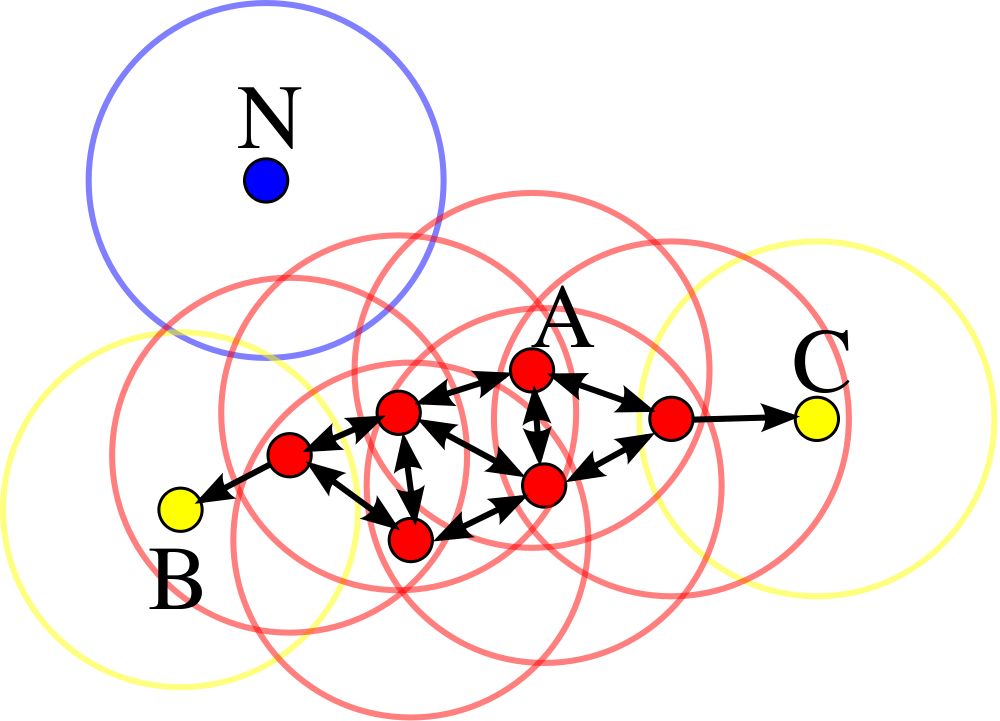
\includegraphics[width=0.8\textwidth]{images/DBSCAN-Illustration.png}
		\caption{Illustration of core points(red), border points(yellow), and outlier(blue)~\cite{wiki:DBSCAN}. In the illustration, $MinPts = 4$, $Eps$ is the radius of those circles.}
		\label{fig:DBSCANConcept}
	\end{center}
\end{figure}

As show in the figure, red points are core points since in each red circle, there are at least 4 points(including the center point). While for the yellow point, they don't have enough points in their circles, but they embed in one of the red circles. Thus, they are border points. As for the blue point, it has neither enough point in the blue cirle nor is in any red circle. Thus, the blue point an outlier/noise.

These definitions reveal the assumption and theory of DBSCAN. DBSCAN assumes that, each cluster consists of two types of points, core points and border points. Core points form inner denser areas compared to spaces outside of clusters. Border points form a slightly sparser areas surrouding the inner core ares, but still the density is higher than spaces between different clusters, possesed by noise. In DBSCAN, the density of an area is measured by the number of points centered at $u$ within an area specified by the given radius $Eps$. If there are at least $MinPts$ points, this area is considered to be a dense area. Thus, this area is part of a cluster. In the procedure \proc{Expand-Cluster}, the algorithm will explore the whole dense area and less dense border area belonging to the same cluster. Each call of \proc{Expand-Cluster} visits a different cluster. Thus, when the whole procedure \proc{DBSCAN} finishes, different clusters are formed.

\subsection{Analysis of DBSCAN}
\label{subsec:DBSCANalgorithm}
DBSCAN applies to a broader range of problems comapred to K-Means. In K-Means, one of the obstacle is to compute the mean value. DBSCAN doesn't have this problem as long as the distance between points is computable. This enables DBSCAN to use more compliated distance measurement, such as edit distance, which is very useful in dealing with strings. Another advantage of DBSCAN is its robustness to noises. As mentioned in section~\ref{subsec:KMeansIssues}, the mean value will be heavily interfere by noises/outliers. In contrast, DBSCAN has a notion noises and it is able to spot these outliers, which is a core problem of this thesis. Finally, the most important advantage of DBSCAN is that it can find arbitrarily shaped clusters. It can even seperate a cluster completely surrounded by a different cluster. An example is shown in Fig~\ref{fig:KMeansDBSCAN}.

\begin{figure}
	\begin{center}
		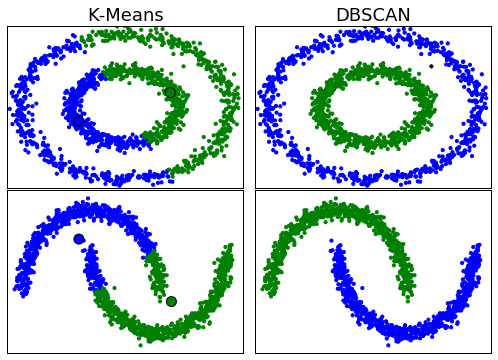
\includegraphics[width=\textwidth]{images/KMeansDBSCAN.png}
		\caption{A Comparison of K-Means and DBSCAN. In the diagram, two datasets ``circles'' and ``moons'' are used. Compared to K-Means, DBSCAN gives more reasonable clustering results on these two irregular shaped datasets.}
		\label{fig:KMeansDBSCAN}
	\end{center}
\end{figure}

Simliar to K-Means, DBSCAN also requires user specified parameters. To get the optimal result, a careful choice of these parameters is needed. Finding the appropriate parameter can be achieved in the similiar way by finding the elbow point as mentioned in section~\ref{subsec:KMeansIssues}. The user can pick a number for $MinPts$ first. Then, for each point, the distance from its $kth$ nearest neighbor is computed. After sorting these distances in descending order and plot them, a graph called \id{sorted k-dist graph} can be obtained. This graph reveals insights about the density distribution of the whole dataset reflected in how the \id{k-dist} varies. Then the $Eps$ can be set to the value corresponding to the elbow point. This heuristic works well as the graph won't differ too much for $k > 4$. An illustration of this approach is shown in Figure~\ref{fig:DBSCANParameter}.~\cite{ester1996density}

\begin{figure}
	\begin{center}
		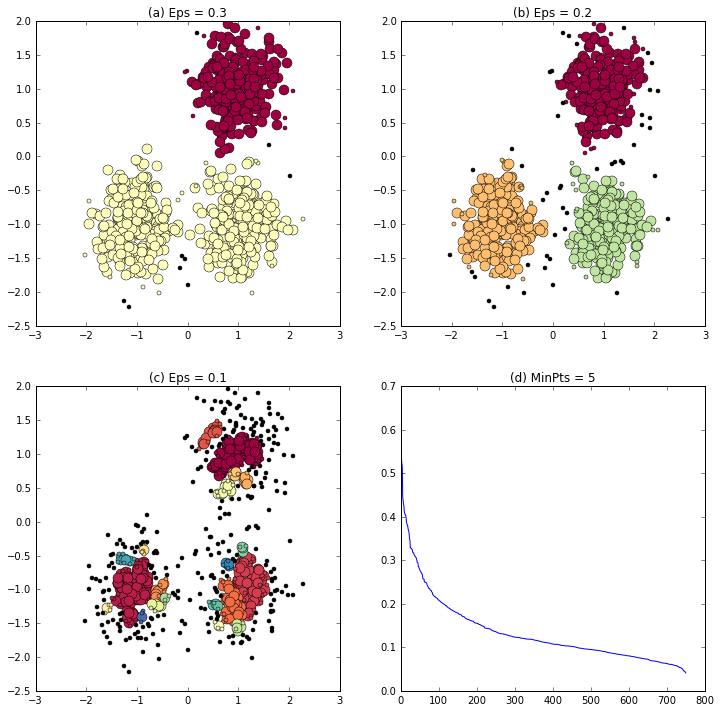
\includegraphics[width=\textwidth]{images/DBSCANParameter.png}
		\caption{Illustration of the heuristic parameter choosing approach for DBSCAN. (a)-(c) illustrates clustering results obtained by using different $Eps$. Each cluster is painted with a different color. Core points are represented using larger circles while border points are represented using smaller circles. Black small circles represent outliers. In figure (a), very few points are labeled as noise and the bottom two clusters are not distinguished. In figure (b), the result is more reasonable and can be considered as optimal. In figure (c), too many points are labeled as noise and more than 3 clusters are reported. According to the \id{k-dist graph} shown in (d), 0.2 should be the best value for $Eps$, which corresponds to the result in figure (b).}
		\label{fig:DBSCANParameter}
	\end{center}
\end{figure}


%When you use \texttt{pdflatex} to render your thesis, you can include PDF images
%directly, as shown by Figure~\ref{fig:indica_model} below.
%
%\begin{figure}[ht]
%  \begin{center}
%    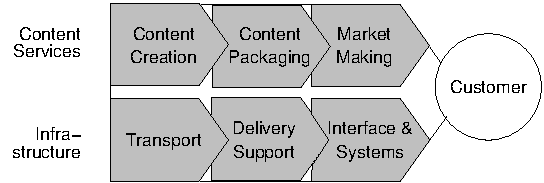
\includegraphics[width=\textwidth]{images/indica_model.pdf}
%    \caption{The INDICA two-layered value chain model.}
%    \label{fig:indica_model}
%  \end{center}
%\end{figure}
%
%You can also include JPEG or PNG files, as shown by Figure~\ref{fig:eeyore}.
%
%\begin{figure}[ht]
%  \begin{center}
%    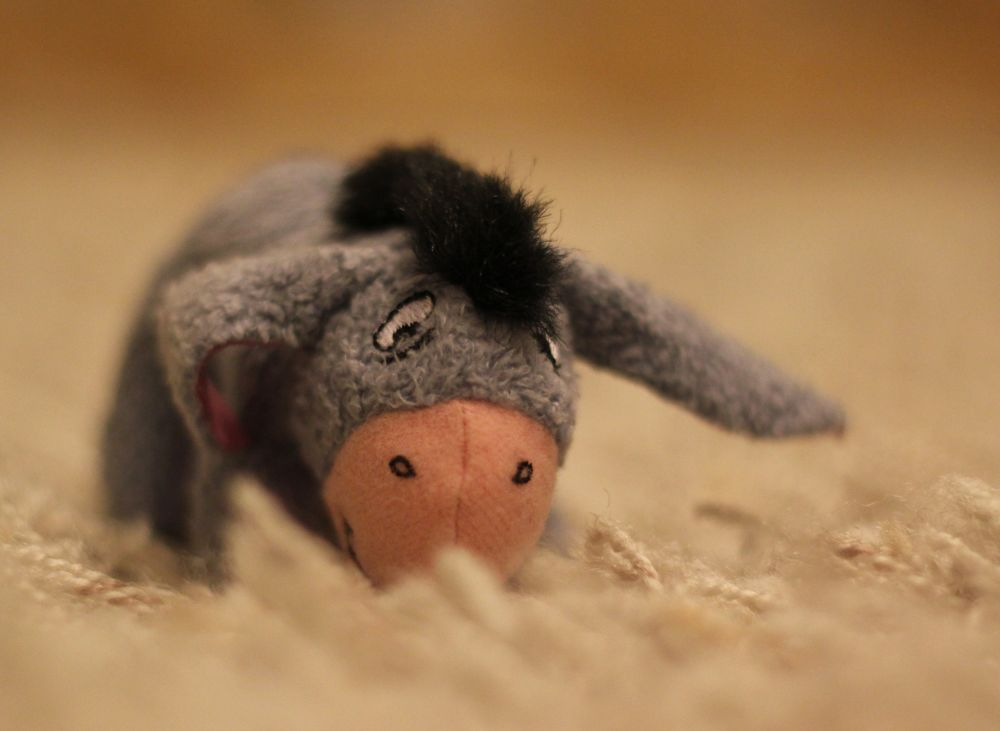
\includegraphics[width=9cm]{images/ihaa.jpg}
%    \caption{Eeyore, or Ihaa, a very sad donkey.}
%    \label{fig:eeyore}
%  \end{center}
%\end{figure}
%
%You can create PDF files out of practically anything.
%In Windows, you can download PrimoPDF or CutePDF (or some such) and install a
%printing driver so that you can print directly to PDF files from any
%application. There are also tools that allow you to upload documents in common
%file formats and convert them to the PDF format.
%If you have PS or EPS files, you can use the tools \texttt{ps2pdf} or
%\texttt{epspdf} to convert your PS and EPS files to PDF\@.
%
%% Comment: If your sentence ends in a capital letter, like here, you should
%% write \@ before the period; otherwise LaTeX will assume that this is not
%% really an end of the sentence and will not put a large enough space after the
%% period. That is, LaTeX assumes that you are (for example), enumerating using
%% capital roman numerals, like I. do something, II. do something else. In this
%% case, the periods do not end the sentence.
%
%% Similarly, if you do need a normal space after a period (instead of
%% the longer sentence separator), use \  (backslash and space) after the
%% period. Like so: a.\ first item, b.\ second item.
%
%Furthermore, most newer editor programs allow you to save directly to the PDF
%format. For vector editing, you could try Inkscape, which is a new open source
%WYSIWYG vector editor that allows you to save directly to PDF\@.
%For graphs, either export/print your graphs from OpenOffice Calc/Microsoft
%Excel to PDF format, and then add them; or use \texttt{gnuplot}, which can
%create PDF files directly (at least the new versions can).
%The terminal type is \emph{pdf}, so the first line of your plot file should be
%something like \texttt{set term pdf \ldots}.
%
%To get the most professional-looking graphics, you can encode them using the
%TikZ package (TikZ is a frontend for the PGF graphics formatting system).
%You can create practically any kind of technical images with TikZ, but it has a
%rather steep learning curve. Locate the manual (\texttt{pgfmanual.pdf}) from
%your \LaTeX\ distribution and check it out. An example of TikZ-generated
%graphics is shown in Figure~\ref{fig:page-merge}.
%
%\begin{figure}[ht]
%  \begin{center}
%    \newcommand*{\actver}{\smash{\ensuremath{v_{\text{\textit{active}}}}}}

\tikzstyle{lbl}=[font=\scriptsize,midway,sloped]
\tikzstyle{opendash}=[densely dotted,thick] 
\tikzstyle{opendeco}=[decoration={zigzag,amplitude=0.1em,segment length=0.6em}]
\tikzstyle{actverline}=[dashed]
\tikzstyle{entryline}=[densely dotted]
\tikzstyle{area}=[ellipse,draw,dashed]
\tikzstyle{liveentry}=[entryline,postaction={%
  decorate,%
  decoration={%
    markings,%
    mark=at position .5pt with{\arrowreversed[line width=.35pt]{|}};,
    mark=at position 1 with{%
      \arrow[line width=.8pt]{stealth}};%
  }%
}]
\tikzstyle{deadentry}=[entryline,postaction={%
  decorate,%
  decoration={%
    markings,%
    mark=at position .5pt with{\arrowreversed[line width=.35pt]{|}};,
    mark=at position 1 with{%
      \arrow[line width=.8pt]{stealth}};%
%      \arrow[line width=.35pt,black,fill=white]{*}};% 
  }%
}]
\tikzstyle{pageborder}=[thick]
\tikzstyle{pagename}=[anchor=center,text=black!50,font=\huge]
\newlength{\spexx}
\setlength{\spexx}{1.2cm}
\newlength{\spexy}
\setlength{\spexy}{.5cm}

\subfigure[Before]{
\begin{tikzpicture}[x=\spexx,y=\spexy,%
  every pin edge/.style={draw,dotted},%
  pin distance=.5\spexx]
  \small
  \coordinate (lo) at (0,-5);
  \coordinate (o) at (0,0);
  \coordinate (hi) at (0,7);
  \coordinate (loact) at (3,-5);
  \coordinate (oact) at (3,0);
  \coordinate (hiact) at (3,7);
  \coordinate (loinf) at (4,-5);
  \coordinate (oinf) at (4,0);
  \coordinate (hiinf) at (4,7);
  
  \draw[->] (lo) -- node[below,lbl] {Versions} ($(loinf) + (1em,0)$);
  \draw[->] (lo) -- node[above,lbl] {Keys} ($(hi) + (0,1em)$);

  \draw[pageborder] (lo) -- (o) -- (hi);
  \draw[pageborder] (lo) -- (loinf);
  \draw[pageborder] (hi) -- (hiinf);
  \draw[pageborder] (o) -- (oinf);

  \draw[opendash] decorate [opendeco] { (loinf) -- (oinf) };
  \draw[opendash] decorate [opendeco] { (oinf) -- (hiinf) };

  \node[pagename] at (2,3.5) {$p$};
  \node[pagename] at (2,-2.5) {$s$};

  \draw[actverline] ($(loact) + (0,-1em)$) node[below=.4em] {\actver} --
    ($(hiact) + (0,1em)$);

  % Page p contents
  \draw[deadentry] (0,6) -- (1,6);
  \draw[deadentry] (1,6) -- (2,6);
  \draw[deadentry] (2,6) -- (3,6);
  \draw[liveentry] (0,5) -- (4,5);
  \draw[deadentry] (0,4) -- (2,4);
  \draw[deadentry] (1,3) -- (3,3);
  \draw[deadentry] (0,2) -- (1,2);
  \draw[deadentry] (2,2) -- (3,2);
  \draw[deadentry] (0,1) -- (2,1);
  \draw[deadentry] (2,1) -- (3,1);

  % Page s contents
  \draw[liveentry] (0,-1) -- (4,-1);
  \draw[deadentry] (0,-2) -- (2,-2);
  \draw[deadentry] (0,-3) -- (3,-3);
  \draw[liveentry] (3,-4) -- (4,-4);

  \node[area,minimum width=4.5\spexx,minimum height=.6\spexy,pin=178:{$1$}]
    at (2,5) {};
  \node[area,minimum width=4.5\spexx,minimum height=.6\spexy,pin=182:{$2$}]
    at (2,-1) {};
  \node[area,minimum width=1.5\spexx,minimum height=.6\spexy,pin=330:{$3$}]
    at (3.5,-4) {};

\end{tikzpicture}}
\subfigure[After]{
\begin{tikzpicture}[x=\spexx,y=\spexy,%
  every pin edge/.style={draw,dotted},%
  pin distance=.5\spexx]
  \small
  \coordinate (lo) at (0,-5);
  \coordinate (o) at (0,0);
  \coordinate (hi) at (0,7);
  \coordinate (loact) at (3,-5);
  \coordinate (oact) at (3,0);
  \coordinate (hiact) at (3,7);
  \coordinate (loinf) at (4,-5);
  \coordinate (oinf) at (4,0);
  \coordinate (hiinf) at (4,7);

  \draw[->] (lo) -- node[lbl,below] {Versions} ($(loinf) + (1em,0)$);
  \draw[->] (lo) -- node[lbl,above] {Keys} ($(hi) + (0,1em)$);

  \draw[pageborder] (lo) -- (o) -- (hi);
  \draw[pageborder] (lo) -- (loinf);
  \draw[pageborder] (hi) -- (hiinf);
  \draw[pageborder] (o) -- (oact);

  \draw[opendash] decorate [opendeco] { (loinf) -- (oinf) };
  \draw[opendash] decorate [opendeco] { (oinf) -- (hiinf) };

  \node[pagename] at (1.5,3.5) {$p$};
  \node[pagename] at (1.5,-2.5) {$s$};
  \node[pagename] at (3.5,1) {$p'$};

  \draw[actverline] ($(loact) + (0,-1em)$) node[below=.4em] {\actver} -- (loact);
  \draw[pageborder] (loact) -- (hiact);
  \draw[actverline] (hiact) -- ($(hiact) + (0,1em)$);

  % Page p contents
  \draw[deadentry] (0,6) -- (1,6);
  \draw[deadentry] (1,6) -- (2,6);
  \draw[deadentry] (2,6) -- (3,6);
  \draw[deadentry] (0,5) -- (3,5);
  \draw[deadentry] (0,4) -- (2,4);
  \draw[deadentry] (1,3) -- (3,3);
  \draw[deadentry] (0,2) -- (1,2);
  \draw[deadentry] (2,2) -- (3,2);
  \draw[deadentry] (0,1) -- (2,1);
  \draw[deadentry] (2,1) -- (3,1);

  % Page s contents
  \draw[deadentry] (0,-1) -- (3,-1);
  \draw[deadentry] (0,-2) -- (2,-2);
  \draw[deadentry] (0,-3) -- (3,-3);

  % Page p' contents
  \draw[liveentry] (3,5) -- (4,5);
  \draw[liveentry] (3,-1) -- (4,-1);
  \draw[liveentry] (3,-4) -- (4,-4);

  \node[area,minimum width=1.5\spexx,minimum height=.6\spexy,pin=10:{$1$}]
    at (3.5,5) {};
  \node[area,minimum width=1.5\spexx,minimum height=.6\spexy,pin=3:{$2$}]
    at (3.5,-1) {};
  \node[area,minimum width=1.5\spexx,minimum height=.6\spexy,pin=330:{$3$}]
    at (3.5,-4) {};
\end{tikzpicture}}

%    \caption{Example of a multiversion database page merge. This figure has
%    been taken from the PhD thesis of Haapasalo~\cite{HaapasaloThesis}.}
%    \label{fig:page-merge}
%  \end{center}
%\end{figure}
%
%Another example of graphics created with TikZ is shown in
%Figure~\ref{fig:tikz-examples}.
%These show how graphs can be drawn and labeled.
%You can consult the example images and the PGF manual for more examples of what
%kinds figures you can draw with TikZ.
%
%% These definitions are only used in the example images; you will not
%% need them for your thesis...
%\newlength{\graphdotsize}
%\setlength{\graphdotsize}{1.7pt}
%\newlength{\graphgridsize}
%\setlength{\graphgridsize}{1.2em}
%\begin{figure}[ht]
%\begin{center}
%\subfigure[Examples of obstruction graphs for the Ferry Problem]{
%  \newlength{\oggs}
\setlength{\oggs}{1.2\graphgridsize}
\begin{tikzpicture}[x=\oggs,y=\oggs,every pin edge/.style={draw,dotted},pin distance=0.5\oggs,area/.style={ellipse,draw,dashed}] 

% The graph (0,0,5,0)
% o = origo
\coordinate (o) at (0,0);
\coordinate[left=1 of o,pin=100:$q_1$] (q1);
\coordinate[right=1 of o,pin=80:$q_2$] (q2);
\fill[black] (q1) circle (\graphdotsize);
\fill[black] (q2) circle (\graphdotsize);
\foreach \d in {-2, -1, ..., 2} {
  \coordinate (tmp) at ($(o) + (0,\d)$);
  \draw (q1) -- (tmp);
  \draw (q2) -- (tmp);
  \fill[black] (tmp) circle (\graphdotsize);
}
\node[area,minimum height=5.3\oggs,minimum width=0.8\oggs,pin=94:$X_3$] at (o) {};  

% The graph (1,0,3,0)
\coordinate[right=5 of o] (o);
\coordinate[left=1 of o,pin=260:$q_1$] (q1);
\coordinate[left=2 of o] (q1v);
\coordinate[right=1 of o,pin=280:$q_2$] (q2);
\fill[black] (q1) circle (\graphdotsize);
\fill[black] (q2) circle (\graphdotsize);
\fill[black] (q1v) circle (\graphdotsize);
\draw (q1) -- (q1v);
\foreach \d in {-1, 0, 1} {
  \coordinate (tmp) at ($(o) + (0,\d)$);
  \draw (q1) -- (tmp);
  \draw (q2) -- (tmp);
  \fill[black] (tmp) circle (\graphdotsize);
}
\node[area,minimum height=3.3\oggs,minimum width=0.8\oggs,pin=266:$X_3$] at (o) {};  
\node[area,minimum height=0.8\oggs,minimum width=0.8\oggs,pin=260:$X_1$] at (q1v) {};  


% The graph (0,1,3,0)
\coordinate[right=4 of o] (o);
\coordinate[left=1 of o,pin=100:$q_1$] (q1);
\coordinate[right=1 of o,pin=80:$q_2$] (q2);
\coordinate[right=2 of o] (q2v);
\fill[black] (q1) circle (\graphdotsize);
\fill[black] (q2) circle (\graphdotsize);
\fill[black] (q2v) circle (\graphdotsize);
\draw (q2) -- (q2v);
\foreach \d in {-1, 0, 1} {
  \coordinate (tmp) at ($(o) + (0,\d)$);
  \draw (q1) -- (tmp);
  \draw (q2) -- (tmp);
  \fill[black] (tmp) circle (\graphdotsize);
}
\node[area,minimum height=3.3\oggs,minimum width=0.8\oggs,pin=94:$X_3$] at (o) {};  
\node[area,minimum height=0.8\oggs,minimum width=0.8\oggs,pin=80:$X_2$] at (q2v) {};  

% The graph (0,0,3,1)
\coordinate[right=5 of o] (o);
\coordinate[left=1 of o,pin=260:$q_1$] (q1);
\coordinate[right=1 of o,pin=290:$q_2$] (q2);
\fill[black] (q1) circle (\graphdotsize);
\fill[black] (q2) circle (\graphdotsize);
\draw (q1) -- (q2);
\foreach \d in {-1, 1, 2} {
  \coordinate (tmp) at ($(o) + (0,\d)$);
  \draw (q1) -- (tmp);
  \draw (q2) -- (tmp);
  \fill[black] (tmp) circle (\graphdotsize);
}
\node[area,minimum height=4.3\oggs,minimum width=0.8\oggs,pin=266:$X_3$] at ($(o) + (0,0.5)$) {};  

\end{tikzpicture}

%}
%\subfigure[Examples of star graphs]{
%  \begin{tikzpicture}[x=\graphgridsize,y=\graphgridsize] 

\coordinate (o) at (0,0);
\fill[black] (o) circle (\graphdotsize);
\foreach \d in {0, 90, ..., 270} {
  \coordinate (tmp) at ($(o) + (\d:1.5)$);
  \draw (o) -- (tmp);
  \fill[black] (tmp) circle (\graphdotsize);
}

\coordinate[right=4 of o] (o);
\coordinate (o1) at ($(o) + (0:0.3)$);
\coordinate (o2) at ($(o) + (180:0.3)$);
\fill[black] (o1) circle (\graphdotsize);
\fill[black] (o2) circle (\graphdotsize);
\draw (o1) -- (o2);
\foreach \d in {45, 135, 270} {
  \coordinate (tmp\d) at ($(o) + (\d:1.5)$);
  \draw (o2) -- (tmp\d);
  \fill[black] (tmp\d) circle (\graphdotsize);
}
\draw (o1) -- (tmp45);


\coordinate[right=4 of o] (o);
\coordinate (o1) at ($(o) + (0:0.3)$);
\coordinate (o2) at ($(o) + (180:0.3)$);
\fill[black] (o1) circle (\graphdotsize);
\fill[black] (o2) circle (\graphdotsize);
\draw (o1) -- (o2);
\foreach \d in {45, 135, 270} {
  \coordinate (tmp\d) at ($(o) + (\d:1.5)$);
  \draw (o2) -- (tmp\d);
  \fill[black] (tmp\d) circle (\graphdotsize);
}
\draw (o1) -- (tmp45);
\draw (o1) -- (tmp135);


\coordinate[right=4 of o] (o);
\coordinate (o1) at ($(o) + (0:0.3)$);
\coordinate (o2) at ($(o) + (180:0.3)$);
\fill[black] (o1) circle (\graphdotsize);
\fill[black] (o2) circle (\graphdotsize);
\draw (o1) -- (o2);
\foreach \d in {45, 135, 270} {
  \coordinate (tmp\d) at ($(o) + (\d:1.5)$);
  \draw (o1) -- (tmp\d);
  \draw (o2) -- (tmp\d);
  \fill[black] (tmp\d) circle (\graphdotsize);
}


\coordinate[right=3.5 of o] (o);
\coordinate (o1) at ($(o) + (90:0.3)$);
\coordinate (o2) at ($(o) + (210:0.5)$);
\coordinate (o3) at ($(o) + (330:0.5)$);
\fill[black] (o1) circle (\graphdotsize);
\fill[black] (o2) circle (\graphdotsize);
\fill[black] (o3) circle (\graphdotsize);
\draw (o1) -- (o2);
\draw (o1) -- (o3);
\draw (o2) -- (o3);
\foreach \d in {90, 270} {
  \coordinate (tmp\d) at ($(o) + (\d:1.5)$);
  \draw (o2) -- (tmp\d);
  \draw (o3) -- (tmp\d);
  \fill[black] (tmp\d) circle (\graphdotsize);
}
\draw (o1) -- (tmp90);


\coordinate[right=3 of o] (o);
\coordinate (o1) at ($(o) + (90:0.3)$);
\coordinate (o2) at ($(o) + (210:0.5)$);
\coordinate (o3) at ($(o) + (330:0.5)$);
\fill[black] (o1) circle (\graphdotsize);
\fill[black] (o2) circle (\graphdotsize);
\fill[black] (o3) circle (\graphdotsize);
\draw (o1) -- (o2);
\draw (o1) -- (o3);
\draw (o2) -- (o3);
\foreach \d in {90, 270} {
  \coordinate (tmp\d) at ($(o) + (\d:1.5)$);
  \draw (o2) -- (tmp\d);
  \draw (o3) -- (tmp\d);
  \fill[black] (tmp\d) circle (\graphdotsize);
}
\draw (o1) -- (tmp90);
\draw (o1) -- (tmp270);



\coordinate[right=3.5 of o] (o);
\coordinate (o1) at ($(o) + (18:1.3)$);
\coordinate (o2) at ($(o) + (90:1.3)$);
\coordinate (o3) at ($(o) + (162:1.3)$);
\coordinate (o4) at ($(o) + (234:1.3)$);
\coordinate (o5) at ($(o) + (306:1.3)$);
\foreach \d in {1, 2, ..., 5} {
  \fill[black] (o\d) circle (\graphdotsize);
}
\draw (o1) -- (o2);
\draw (o1) -- (o3);
\draw (o1) -- (o4);
\draw (o1) -- (o5);
\draw (o2) -- (o3);
\draw (o2) -- (o4);
\draw (o2) -- (o5);
\draw (o3) -- (o4);
\draw (o3) -- (o5);
\draw (o4) -- (o5);

\end{tikzpicture}

%}
%\caption{Examples of graphs draw with TikZ. These figures have been taken from a
%course report for the graph theory course~\cite{FerryProblem}.}
%\label{fig:tikz-examples}
%\end{center}
%\end{figure}


\chapter{Scoring Patient Visits by Markov Models}
%MM: mention sequential data
%HMM, advantages: more complex dependence, enable contruction from simpler blocks
\label{chapter:generative}
This chapter is going to explore generative methods for anomaly detection. Generative methods are a collection of algorithms which try to build a model that explains the process of how the data generates. Then, the model gives a score indicating how likely one entry is an anomaly. A family of algorithms belonging to this category is the Markov models~\cite{isaacson1976markov}.

The patients visits can be seen as time sequential data consisting of a series of events. The events in one visit are not generated independently and randomly. Instead, past events have an effect on the type of the next possible event. To handle sequential data, Markov models are good choices since they consider the relation between consecutive observations. In the following context, Section~\ref{sec:MM} introduces the basic Markov chain model. Later, Section~\ref{sec:HMM} expands the Markov chain to a more complicated Hidden Markov Model by introducing hidden variables.

\section{Discrete Markov Process}
\label{sec:MM}
Consider a system having \(K\) distinct states \(\{s_1, s_2, \cdots, s_K\}\). At any time, the system will be in one of these states. After a given time period \(N\), a series observation \(\{x_1, x_2, \cdots, x_N\}\), where $x_n \in \{s_1, s_2, \cdots, s_K\}$, can be obtained. (Without loss of generality, the following discussion assumes the variables are all scalar. The assumption holds in the rest of the context unless explicitly stated otherwise) According to the product rule of probability, the joint probability distribution for this sequence of observations is
\begin{equation}
	p(x_1, x_2, \cdots, x_T) = \prod_{n = 2}^{N} p(x_n \mid x_1, \cdots, x_{n-1})
\end{equation}

The conditional probability distribution of each observation \(x_n\) depends on all observations having a smaller index than it. The above relations between the observations can be represented graphically in Figure~\ref{fig:MM}(a). The graph is fully connected, and no independence property can be obtained from it. Now assume that each observation \(x_n\) only depends on one immediate previous observation \(x_{n-1}\). Then the joint distribution becomes 
\begin{equation}
	p(x_1, x_2, \cdots, x_N) = p(x_1)\prod_{n = 2}^{N} p(x_n \mid x_{n-1})
\end{equation}
This newly obtained model is depicted in Figure~\ref{fig:MM}(b), and is referred as \textit{first-order Markov chain}. The term \textit{first-order} indicates the dependence on only one previous observation. Suppose the system has only 3 states, as shown in Figure~\ref{fig:MM}(c). Then, to fully represent the system, the only required information is the transition probabilities between different sates. The transition probabilities are usually referred as \textit{transition matrix}, denoted as \(\mathbf{A}\). Each element \(A_{ij}\) represents the probability of transferring from state \(s_i\) to state \(s_j\). Learning the parameters of this model is very simple. Since the states are exactly the observations, \(A_{ij}\) can be simply obtained by compute the frequency of transferring to \(s_j\) starting from \(s_i\). The number of free parameters in this model is \(K(K-1)\), where \(K\) represents the number of states in the system.

\begin{figure}[!ht]
	\begin{center}
		\includegraphics[scale = 0.75]{images/MM.png}
		\caption{Illustration of a Markov Chain of 4 observations possessing 3 states. Variables are represented using filled circles, while states are represented using filled squares. Variable value can be only from $\{s_1, s_2, s_3\}$.}
		\label{fig:MM}
	\end{center}
\end{figure}

Sometimes, the observations can depend on more than one observations in the past. One simple way to achieve this is creating a higher order Markov chain. By allowing each observation to depend on previous two values, a second-order Markov chain is obtained, as shown in Figure~\ref{fig:secondOrderMM}. Then the joint distribution becomes
\begin{equation}
	p(x_1, x_2, \cdots, x_N) = p(x_1)p(x_2 \mid x_1)\prod_{n = 3}^{N} p(x_n \mid x_{n-1}, x_{n-2})
\end{equation}
Using the same state space representation, the \textit{second-order Markov chain} has better capability of modelling complex relations between variables, compared to \textit{first-order Markov chain}. In fact, the higher the order is, the more flexible the model is. However, the number of parameters grows as well, which makes the model difficult to train. For a \(M^{th}\)-order Markov Chain, there will be \(K^{M}(K-1)\) parameters. Because the exponential growth in number of parameters, the model gradually becomes impractical as \(M\) grows. 

\begin{figure}[!ht]
	\begin{center}
		\includegraphics[scale=0.8]{images/secondOrderMM}
		\caption{Illustration of a second-order Markov model.}
		\label{fig:secondOrderMM}
	\end{center}
\end{figure}


\section{Hidden Markov Model}
\label{sec:HMM}
The simple Markov Chain model is not enough for modelling the patient visit sequence. The variables \(\{x_1, x_2, \cdots, x_N\}\) can be considered as the patient states, namely \texttt{ENROLLING}, etc. However, the visit sequence also contains time part. To integrate the time part into the model, the Markov Chain model can be expanded in another way, by associating an emission distribution \(\mathbf{E}_k\), \(k = 1, \cdots , K\), to each state in the system. Thus, two observations \(x_n\), \(y_n\) exist at any time, where \(y_n\) is generated depending on \(x_n\). If the relation between \(\{x_1, x_2, \cdots, x_N\}\) is modelled as a first-order Markov chain, the joint distribution becomes
\begin{equation}
	p(x_1, y_1, \cdots, x_N, y_N) = p(x_1) \prod_{n = 2}^{N} p(x_n \mid x_{n-1}) \prod_{n = 1}^{N}p(y_n|x_n)
\end{equation}
where \(x_t\) represents the patient state and \(y_t\) represents the associated duration. For each visit, the patient goes through a series of events, which is the patient state. Each event will then last for a certain period of time. The duration can be seen as generated from a distribution, and the parameters of this distribution depend on the event. One example is shown in Figure~\ref{fig:patientMM}. This model is in fact a special case of Hidden Markov Model. This section explores Hidden Markov Model in details.

\begin{figure}[!ht]
	\begin{center}
		\includegraphics[width=0.8\textwidth]{images/patientMM}
		\caption{Modelling a patient visit as a special case of Hidden Markov Model.}
		\label{fig:patientMM}
	\end{center}
\end{figure}

\subsection{Definition of Hidden Markov Model}
As mentioned in the last section, a trade-off between flexibility and practicality exists in deciding the order number for a Markov chain model. It would be ideal if a model is not limited to any specific given order, and still only limited number of parameters are required to specify the model. Luckily, these requirements can be satisfied by constructing a Hidden Markov Model using additional latent variables~\cite{PRML}. 

Suppose a sequence of observations \(\mathbf{X} = \{x_1, \cdots, x_N\}\) is obtained. Instead of assuming each observation depends directly on a specific number of previous observations, the new assumption is that, there is a latent variable \(z_t\) corresponding to each observation, and the latent variables form a Markov chain. The latent variables don't have to possess any physical meanings. They can even be of different type to the observations, in terms of distribution and dimensionality. A graphical representation of this model is shown in Figure~\ref{fig:HMM}. It's easy to get confused by comparing Figure~\ref{fig:patientMM} and Figure~\ref{fig:HMM} since they share the same graphical structure. The difference is that, in Figure~\ref{fig:HMM}, the \(z_t\)'s are unobserved latent variables, which is depicted using unfilled circles, while in Figure~\ref{fig:patientMM}, both events and duration are observed values. All observed variables are represented using filled circles. Despite the fact there are no unobserved variables in Figure~\ref{fig:patientMM}, it still belongs to HMM family. In this model, we just happen to observe all variables. It is possible to add additional latent variables into this model. One potential structure could be the one shown in Figure~\ref{fig:patientHMM}. Intuitively, in this model, the value of the newly added latent variable determines which event will generate, then the event determines how long the duration will be. Notice that the latent variables don't have any associated physical meaning or specific distribution form. One can explain them as indication of the functioning status of the system by selecting them to be binary variables. When \(z_t\) = 1, it indicates the queue system in the hospital is working in normal mode. When \(z_t\) = 0, it means the system is working in a problematic way. A similar model has been proposed by Hollm\'en and Tresp~\cite{hollmen2000hidden}.

\begin{figure}[!ht]
	\begin{center}
		\includegraphics[scale = 0.8]{images/HMM}
		\caption{Graphical representation of a Hidden Markov Model. Observations are represented using filled circles, while latent variables are depicted using unfilled circles. The latent variables form a first-order Markov chain.}
		\label{fig:HMM}
	\end{center}
\end{figure}

\begin{figure}[!ht]
	\begin{center}
		\includegraphics[width=0.8\textwidth]{images/patientHMM}
		\caption{Modelling patient visit as Hidden Markov Model. Event types and event duration are represented using filled eclipses and circles respectively. Additional hidden variables are represented using unfilled circles. No specific physical meaning is associated with these latent variables.}
		\label{fig:patientHMM}
	\end{center}
\end{figure}

In the framework of HMM, the joint distribution over both observed and latent variables is given below
\begin{equation}
	p(\mathbf{X}, \mathbf{Z} | \boldsymbol{\theta}) = p(z_1 | \pi) \prod_{n=2}^{N}p(z_n\mid z_{n-1}, \mathbf{A}) \prod_{m=1}^{N}p(x_m\mid z_m, \phi)
	\label{eq:HMMcomplete}
\end{equation}
where \(\mathbf{X} = \{x_1, \cdots, x_N\}\) represents all the observed variables, \(\mathbf{Z} = \{z_1, \cdots, z_N\}\) represents latent variables, and \(\boldsymbol{\theta} = \{\pi, \mathbf{A}, \phi\}\) represents the parameters in this model. The \(\pi\) is a prior distribution for deciding the value of the first variable \(z_1\). The matrix \(\mathbf{A}\) is the transition matrix among the latent variables. The \(\phi\) are the parameters of the emission distribution associated with \(z_t\) and \(x_t\).

\subsection{Learning and Inference}
There are three basic problems in HMM.~\cite{rabiner1989tutorial}  These problems are described below using above notations:
\begin{itemize}
	\item Problem 1: Given a sequence of observations \(\mathbf{X} = \{x_1, \cdots, x_N\}\), what is the probability \(p(\mathbf{X} | \boldsymbol{\theta}) 			  \)over the observations, under specific parameters \(\boldsymbol{\theta} = \{\pi, \mathbf{A}, \phi\}\)?
	\item Problem 2: What's the value of the parameters which maximizes the likelihood \(p(\mathbf{X} | \boldsymbol{\theta})\)?
	\item Problem 3: Given a sequence of observations \(\mathbf{X} = \{x_1, \cdots, x_N\}\), what is the value of the corresponding latent variables?
\end{itemize}
If luxury of observing the latent variable is available, these three problems becomes trivial. But if we do not have this luxury, these three problems become complicated. The rest of the context focus on the first two questions, assuming the latent variable are unobservable. The reason is that, once the value of \(p(\mathbf{X} | \boldsymbol{\theta})\) is computed, the decision on whether a given sequence is anomaly can be made by comparing \(p(\mathbf{X} | \boldsymbol{\theta})\) to a threshold value.

Though it seems more intuitive that finding a way to evaluate \(p(\mathbf{X} | \boldsymbol{\theta})\) should come before maximizing it with respect to the parameters, it would be more convenient to start at solving problem 2. After solving problem 2, the solution to the first problem will appear naturally. The following discussion begins by introducing some new concepts and notations.

The distribution over only observed variables \(p(\mathbf{X} | \boldsymbol{\theta})\) is usually referred as \textit{incomplete likelihood}, while distribution over both observed and unobserved variables \(p(\mathbf{X}, \mathbf{Z} | \boldsymbol{\theta})\) is referred as \textit{complete likelihood}. Using Equation~\ref{eq:HMMcomplete}, the logarithm of incomplete likelihood can be represented as
\begin{equation}
	\begin{split}
		\ln p(\mathbf{X} | \boldsymbol{\theta}) & = \ln \sum_{\mathbf{Z}}p(\mathbf{X}, \mathbf{Z} | \boldsymbol{\theta}) \\
										   & = \ln p(z_1 | \pi)  + \ln \sum_{\mathbf{Z}}\Big( \prod_{n=2}^{N}p(z_n\mid z_{n-1}, \mathbf{A}) \prod_{m=1}^{N}p(x_m\mid z_m, \phi)\Big)
	\end{split}
\end{equation}
The above equation is a generalization of the \textit{mixture distribution}~\cite{PRML}. Maximizing $\ln p(\mathbf{X} | \boldsymbol{\theta})$ with respect to the parameters is very difficult since the derivatives don't have a closed form. An alternative practical working algorithm is the \textit{expectation-maximization(EM)} algorithm~\cite{dempster1977maximum}\cite{mclachlan2007algorithm}. The EM algorithm is very similar to the K-Means algorithm mentioned in Chapter~\ref{chapter:clustering}. The algorithm consists of two steps, E-step and M-step. In the E-step, the algorithm fixes the value of parameters and find the posterior distribution of the latent variables \(p(\mathbf{Z} | \mathbf{X}, \boldsymbol{\theta}^{old})\). Here the notation is adopted from Bishop's~\cite{PRML}. The superscription \textit{old} in \(\theta^{old}\) means the parameter is fixed. Then the algorithm computes the expectation of the logarithm of the complete likelihood, with respect to the derived posterior distribution. The newly derived term becomes a function of \(\boldsymbol{\theta}\), which is shown below
\begin{equation}
	Q(\boldsymbol{\theta}, \boldsymbol{\theta}^{old}) = \sum_{\mathbf{Z}}p(\mathbf{Z}| \mathbf{X}, \boldsymbol{\theta}^{old})\ln p(\mathbf{X}, \mathbf{Z} | \boldsymbol{\theta})
\end{equation}
Then in the M-step,  the new value of \(\boldsymbol{\theta}\) is updated by maximizing \(Q(\boldsymbol{\theta}, \boldsymbol{\theta}^{old})\). Compared to K-Means, the E-step corresponds to assign each point to a cluster prototype, and the M-step corresponds to update the value of the prototypes. These two steps are executed alternatively until convergence or maximum number of iteration is reached. In the following text, \(\gamma(\mathbf{z}_n)\) and \(\gamma(\mathbf{z}_{n-1}, \mathbf{z}_n)\) are introduced which stand for the posterior distribution of a single latent variable and the joint posterior distribution over two consecutive latent variables, separately. Instead of assuming the latent variables are scalar, here they are represented using \textit{1-of-K} coding. Namely, each latent variable is a length \(K\) vector, where one and only one of these \(K\) elements equals 1. When \(z_{nk} = 1\), it means the \(nth\) latent variable is in the \(kth\) state. Using this representation schema, following equations are obtained~\cite{PRML}
\begin{align}
	\gamma(\mathbf{z}_n) = &p(\mathbf{z}_n | \mathbf{X}, \boldsymbol{\theta}^{old})	\\
	\gamma(\mathbf{z}_{n-1}, \mathbf{z}_n) = &p(\mathbf{z}_{n-1}, \mathbf{z}_n | \mathbf{X}, \boldsymbol{\theta}^{old}) \\
	Q(\boldsymbol{\theta}, \boldsymbol{\theta}^{old}) = &\sum_{k=1}^{K} \gamma(z_{1k})\ln \pi_k + \sum_{n=2}^{N}\sum_{j=1}^{K}\sum_{k=1}^{K}\gamma(\mathbf{z}_{n-1}, \mathbf{z}_n)\ln A_{jk}		\notag		\\
		&+ \sum_{n=1}^{N}\sum_{k=1}^{K}\gamma(z_{nk})\ln p(x_n|\phi_k)	
\end{align}

Computation in the M-step is relatively easy. Assume the E-step has been done, so that  \(\gamma(\mathbf{z}_n)\) and \(\gamma(\mathbf{z}_{n-1}, \mathbf{z}_n)\) are like constants now. Then following update equation can be obtained
\begin{align}
	\pi_k = & \frac{\gamma(z_{1k})}{\sum_{j=1}^{K}\gamma(z_{1j})}	\\
	A_{jk} = & \frac{\sum_{n=2}^{N}\gamma(z_{n-1,j},z_{nk})}{\sum_{l=1}^{K}\sum_{n=2}^{N}\gamma(z_{n-1,j},z_{nl})}
\end{align}
Update of \(\phi_k\) is more tricky, since it depends on the specific choice of the emission distribution. One good observation is that, only the final term depends on \(\phi_k\), and different \(\phi_k\) doesn't couple with each other. Thus, each \(\phi_k\) can be updated separately. The term \(\gamma(z_{nk})\) functions as a soft assignment, representing the probability of assigning a point \(x_n\) to each state.

Computation in E-step is more difficult which requires efficient algorithm. The most widely used algorithm is known as \textit{alpha-beta} algorithm. This algorithm can be seen as an application of dynamic programming technique which takes advantage of the tree structure in HMM thus leading to efficiency. To start with the alpha-beta algorithm, following conditional independence properties should be obtained first~\cite{jordan2003introduction}
\begin{align}
	p(\mathbf{X}| \mathbf{z}_n) = &p(x_1, \cdots, x_n | \mathbf{z}_n)	\notag \\	
										&p(x_{n+1}, \cdots, x_N | \mathbf{z}_n) \\
	p(x_1, \cdots, x_{n-1}| x_n, \mathbf{z}_n) = &p(x_1, \cdots, x_{n-1} | \mathbf{z}_n)	\\
	p(x_1, \cdots, x_{n-1}| z_{n-1}, \mathbf{z}_n) = &p(x_1, \cdots, x_{n-1} | \mathbf{z}_{n-1})
\end{align}
These equations can be obtained by using \textit{d-seperation} technique~\cite{pearl2014probabilistic}, or proved formally using sum and product rules of probability. Using the first independence property and Bayes' theorem, following equations are obtained
\begin{equation}
	\label{eq:gammaZn}
	\begin{split}
	\gamma(\mathbf{z}_n) &= p(\mathbf{z}_n | \mathbf{X})  = \frac{p(\mathbf{X}| \mathbf{z}_n)p(\mathbf{z}_n)}{p(\mathbf{X})}	\\
										 & = \frac{p(x_1, \cdots, x_n, \mathbf{z}_n)p(x_{n+1}, \cdots, x_N | \mathbf{z}_n)}{p(\mathbf{X})}	\\
										 & = \frac{\alpha(\mathbf{z}_n)\beta(\mathbf{z}_n)}{p(\mathbf{X})}
	\end{split}
\end{equation}
where
\begin{align}
	\alpha(\mathbf{z}_n) & = p(x_1, \cdots, x_n, \mathbf{z}_n)\\
	\beta(\mathbf{z}_n)  & = p(x_{n+1}, \cdots, x_N | \mathbf{z}_n)
\end{align}
Using the other two conditional independence properties, \(\alpha(\mathbf{z}_n)\) can be expressed recursively in terms of \(\alpha(\mathbf{z}_{n-1})\)
\begin{equation}
	\begin{split}
	\alpha(\mathbf{z}_n) &=  p(x_n | \mathbf{z}_n) \sum_{\mathbf{z}_{n-1}}p(x_1, \cdots, x_{n-1}, \mathbf{z}_{n-1})p(\mathbf{z}_n | \mathbf{z}_{n-1}) \\
						 &=  p(x_n | \mathbf{z}_n) \sum_{\mathbf{z}_{n-1}} \alpha(\mathbf{z}_{n-1})p(\mathbf{z}_n | \mathbf{z}_{n-1})
	\end{split}
\end{equation}
Similarly, \(\beta(\mathbf{z}_n)\) can also be expressed recursively as
\begin{equation}
	\beta(\mathbf{z}_n) = \sum_{\mathbf{z}_{n+1}}\beta(\mathbf{z}_{n+1})p(x_{n+1}|\mathbf{z}_{n+1})p(\mathbf{z}_{n+1}|\mathbf{z}_n)
\end{equation}
The term \(\alpha(\mathbf{z}_n)\) can be seen as messages propagated from the beginning to the end. Each \(\alpha(\mathbf{z}_n)\) receives messages passed from its predecessor, combines these information with its own information and then pass them to its successor. The logical also applies to the term \(\beta(\mathbf{z}_n)\), but the messages are from the end to the beginning. Due to the tree structure in HMM, computing each term only depends on one adjacent term, instead of all terms before/after it. Thus, the computation reduces dramatically which makes the algorithm efficient. To start the whole computation, initial conditions \(\alpha(\mathbf{z}_1)\) and \(\beta(\mathbf{z}_n)\) are required. The initial conditions are given below
\begin{align}
	\alpha(\mathbf{z}_1) &= \prod_{k=1}^{K}\{\pi_k p(x_1 | \phi_k) \}^{z_{1k}}	\\
	\beta(\mathbf{z}_N) &= 1
\end{align}

Having obtained \(\alpha(\mathbf{z}_n)\) and \(\beta(\mathbf{z}_n)\), the posterior distribution \(\gamma(\mathbf{z}_n)\) can be computed as in equation~(\ref{eq:gammaZn}). As for \(\gamma(\mathbf{z}_{n-1}, \mathbf{z}_n)\), it can be computed as following
\begin{align}
\gamma(\mathbf{z}_{n-1}, \mathbf{z}_n) &= p(\mathbf{z}_{n-1}, \mathbf{z}_n | \mathbf{X}) \nonumber \\
									   & = \frac{p(\mathbf{X} | \mathbf{z}_{n-1}, \mathbf{z}_n)p(\mathbf{z}_{n-1}, \mathbf{z}_n)}{p(\mathbf{X})}\nonumber \\
									   & = \frac{p(x_1, \cdots, x_{n-1} | \mathbf{z}_{n-1}) p(x_n | \mathbf{z}_n) p(x_{n+1}, \cdots, x_N | \mathbf{z}_n)
									   			 p(\mathbf{z}_n | \mathbf{z}_{n-1}) p(\mathbf{z}_{n-1})}{p(\mathbf{X})}\nonumber \\
									   & = \frac{\alpha(\mathbf{z}_{n-1}p(x_n|\mathbf{z}_n)p(\mathbf{z}_n|\mathbf{z}_{n-1})\beta(\mathbf{z}_n)}{p(\mathbf{X})}
\end{align}
Up till now, both steps in EM algorithm are introduced, and the problem 2 can be solved efficiently. The left question is how to solve problem 1, computing the likelihood over the incomplete data. The solution comes from  Equation~\ref{eq:gammaZn}. Notice that \(\gamma(\mathbf{z}_n)\) is a posterior distribution. Integrating both sides of Equation~\ref{eq:gammaZn} over \(\mathbf{z}_n\) gives
\begin{equation}
	p(\mathbf{X}) = \sum_{\mathbf{z}_n} \alpha(\mathbf{z}_n)\beta(\mathbf{z}_n)
\end{equation}
where \(\mathbf{z}_n\) is an arbitrary latent variable. If \(n = N\), then \(\beta(\mathbf{z}_n) = 1\), which makes the above equation simpler
\begin{equation}
	p(\mathbf{X}) = \sum_{\mathbf{z}_N} \alpha(\mathbf{z}_N)
\end{equation}
Then, both problem 1 and problem 2 are solved.
 
\chapter{Experiment}
\label{chapter:Experiment}

% what data are used? (period time)
% what preprocess was done? (remove data generated by system)
% how to represent the data? (time sequence)
% how to measure the distance? (modified edit distance)
% Which method to use, why? ( DBSCAN, MM)
	% Can't compute a mean value,	there should be clusters in the data, clustered by department
	% MM is enough. No need to use HMM to complicate the model. Using HMM doesn't explain intuitively, error happened in one phase doesn't lead to error in
	%	the following phase. Different visits don't have direct impact either. Error are usually caused by operators, at least I assume it is this case.
	
This chapter describes the detailed experimental implementation. Following topics will be discussed:
\begin{itemize}
	\item	Which specific data are used? How to represent the data? What preprocess has been done? What related functions are defined?
	\item	Which methods are used? What's the reason to use such methods? 
\end{itemize}
The three topics will be discussed in three sections, respectively. Analysis of the result will be postponed to Chapter~\ref{chapter:evaluation}.

\section{Data Details}
Since the akseli system has gone through several updation after its first release, many features have changed, including how the visit log is reocrded. Considering this aspect, only data generated after year 2014 is retrieved. All the data are from Oulu Hospital, with patient privacy information eliminated. In total, 243K unique visits with 1.93 million entries are retrieved, which spans from January to July. The retrieved data consists of three columns: visit id, event type, and recorded time of the event. Other information, such as which resource generated the data, is not retrieved. Among the retrieved data, 7 event types are adopted. The used event types are: \texttt{ENROLLING}, \texttt{WAITING}, \texttt{IN\_TREATMENT\_ROOM}, \texttt{PAUSED}, \texttt{IN\_TREATMENT\_ROOM\_FROM\_PAUSED}, \texttt{CLOSED}, and \texttt{CANCELLED}.
Inspired by Huang et al~\cite{huang2012anomaly}, a similiar representation form is proposed. In this representation, each patient visit consists of several pairs. Each pair is a combination of event type and duration of being in this event.% Write what is the difference between my representation and huang's. And why is it?

\chapter{Results and Discussion}
\label{chapter:results}
Since the data doesn't have labels indicating which entries are anomalies, precise quantitative evaluation is not possible. To examine how the methods perform, user interpretation of the data is the only standard. To help strengthen intuitive understanding, a visualization method t-SNE\cite{maaten2008visualizing} was applied. This method only requires a distance metric between pairs of data entries. Then it projects the entries into a 2D space showing potential structures underlying the data. t-SNE typically places ``important'' points in the center of the drawing. The concept of ``importance'' can be understand as a special kind of density. Intuitively, points lying in dense area are less likely to be outliers.

Section~\ref{sec:clustering} and ~\ref{sec:generative} describes results obtained using clustering method and generative method respectively. Then, Section~\ref{sec:discuss} compares these two methods.
\section{Clustering Method Results}
\label{sec:clustering}
The first step of applying DBSCAN is to choose parameters. As stated in Section~\ref{subsec:DBSCANalgorithm}, DBSCAN is relatively robust with $k > 4$, where $k$ stands for the $k$th nearest neighbour. In this experiment, $k$ was set to 7. The distance of the $7$th nearest neighbour of all points is draw in Figure~\ref{fig:paramDBSCAN}. The figure shows that the distance begins to increase dramatically beyond 0.5. Thus, in the experiment, $Eps$ was finally set to 0.5, with $MinPts = 7$. The clustering result is shown in Table~\ref{tab:ClusterResult} and visualized in Figure~\ref{fig:ClusterResult}.
\begin{figure}[!ht]
	\begin{center}
		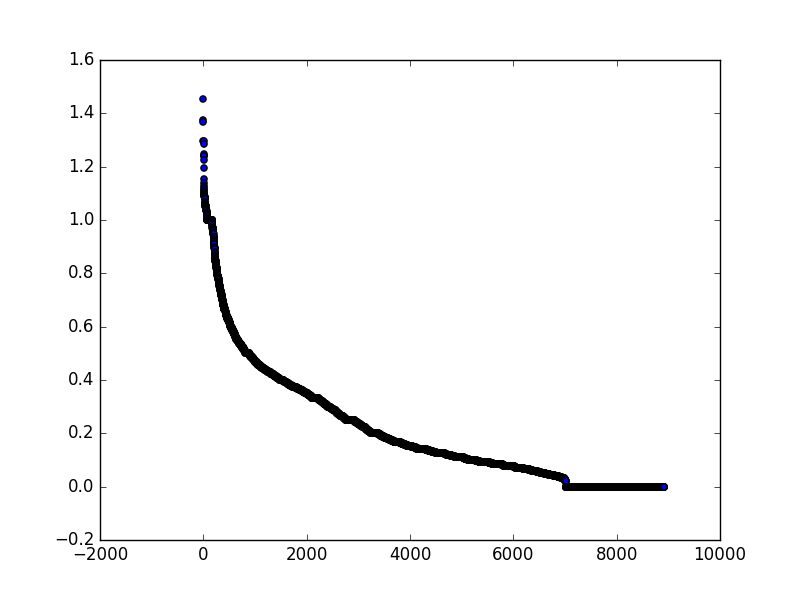
\includegraphics[width=\textwidth]{images/paramDBSCAN}
		\caption{7th nearest neighbour distance for selecting $Eps$ of DBSCAN}
		\label{fig:paramDBSCAN}
	\end{center}
\end{figure}

\begin{table}[!ht]
	\caption{Mean, variance, and dispersion of data generated from largest department.}
	\begin{center}
		\begin{tabular}{|c|c|c|c|c|c|c|c|c|c|c|c|c|}
			\hline
			Cluster No. &    0 & 1  & 2    & 3   & 4   & 5   & 6  & 7   & 8  & 9  & 10 & 11	\\ \hline
			Num Points  &  352 & 10 & 7547 & 134 & 215 & 283 & 64 & 104 & 44 & 47 & 21 & 94 \\
			\hline

		\end{tabular}
	\end{center}
	\label{tab:ClusterResult}
\end{table}

\begin{figure}[!ht]
	\begin{center}
		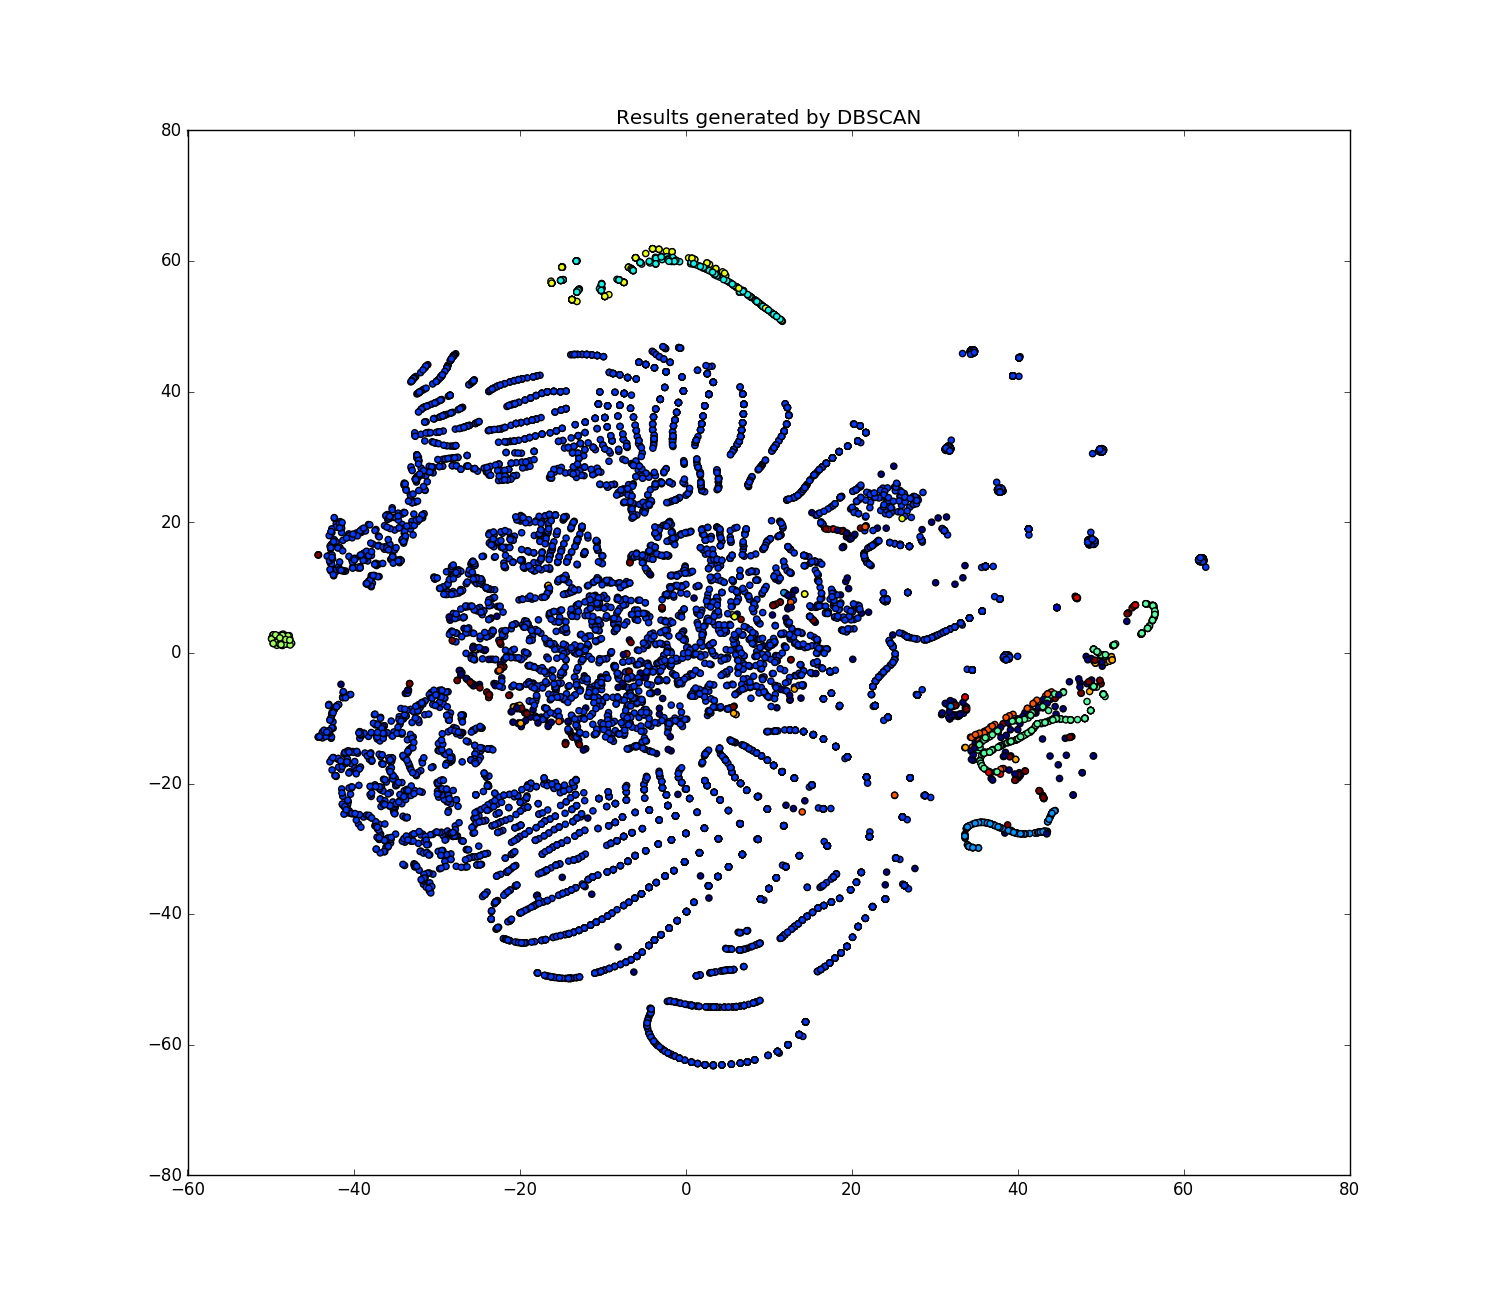
\includegraphics[width=\textwidth]{images/ClusterResult}
		\caption{Results generated by DBSCAN, visualized using t-SNE. All clusters are shown. Each cluster is plotted in a different color.}
		\label{fig:ClusterResult}
	\end{center}
\end{figure}

\begin{figure}[!ht]
	\begin{center}
		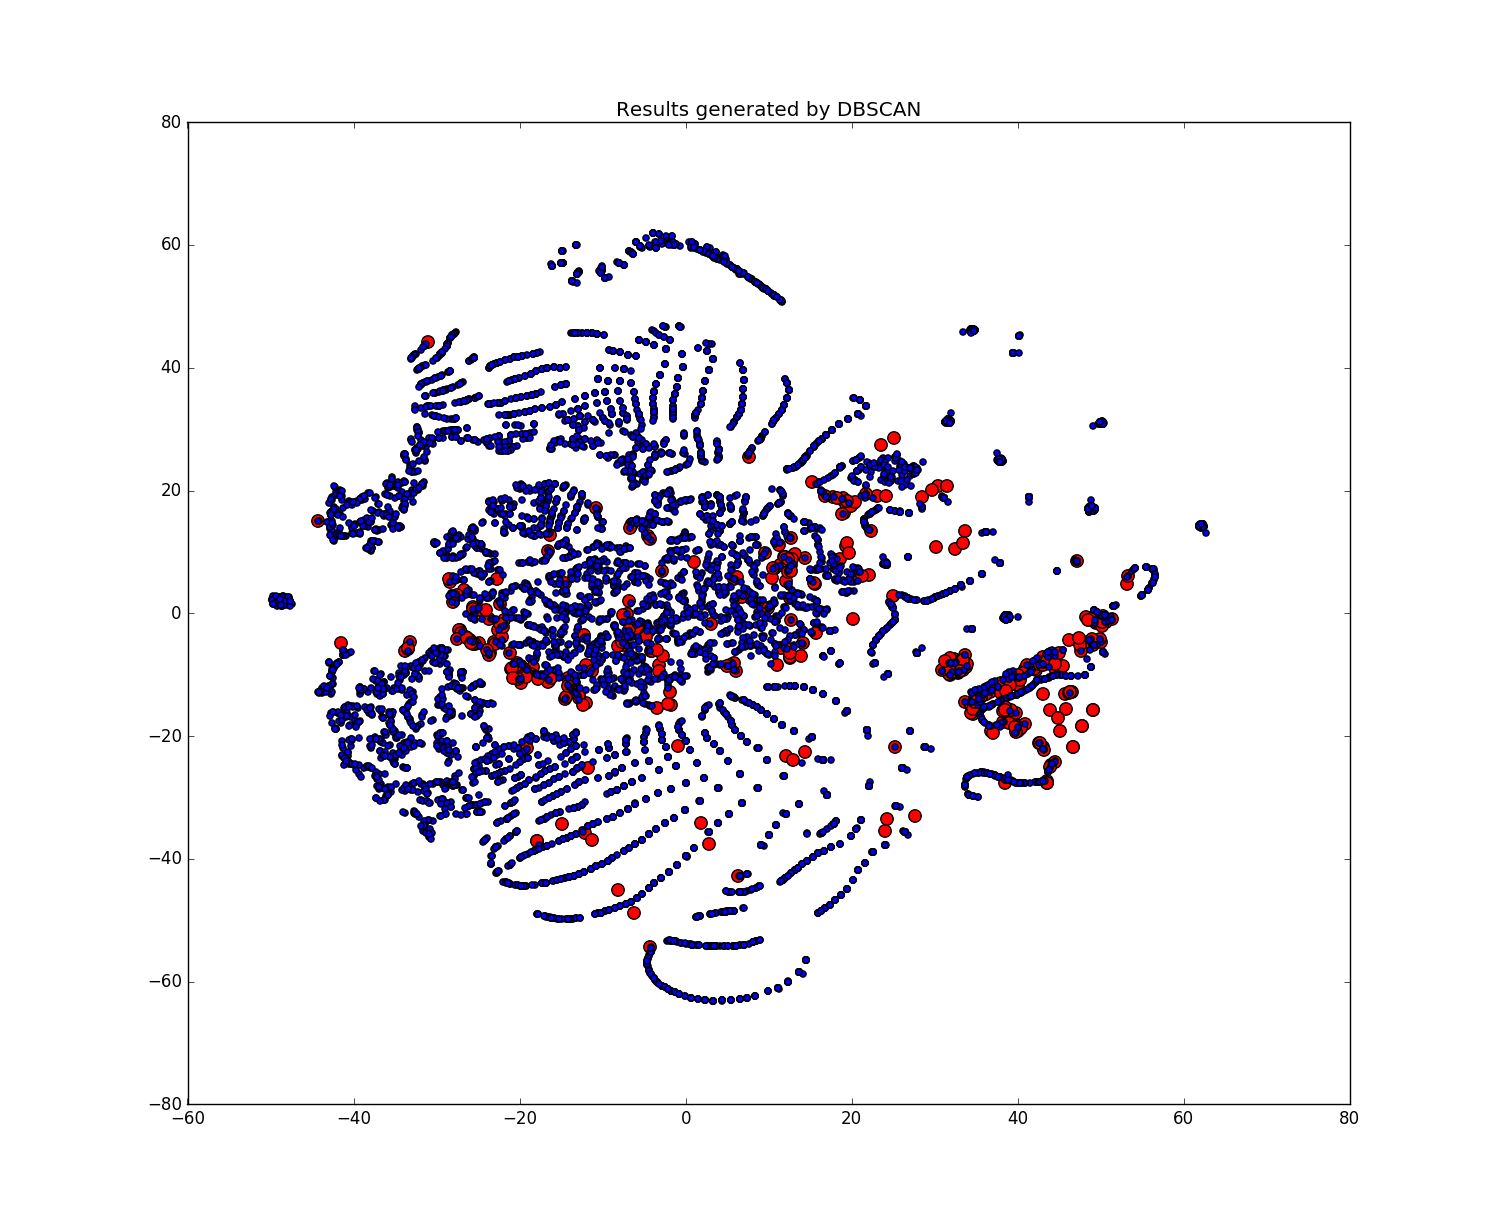
\includegraphics[width=\textwidth]{images/ClusterResult2}
		\caption{Results generated by DBSCAN, visualized using t-SNE. Cluster 0 is plotted in red, while all the rest clusters are plotted in blue.}
		\label{fig:ClusterResult2}
	\end{center}
\end{figure}

As shown in the table, 12 clusters are generated by DBSCAN. Among the 12 clusters, cluster 0 is labelled as noise/anomalies which consists of 352 visits. Cluster 2 is the largest cluster which consists of 7547 visits. This cluster is believed to consists of the most typical visits. For the rest small clusters, they can be considered as representing some non-typical but normal visits. One potential reason of generating such sub-clusters is that, there are many different resources/machines for diagnosing. Data in these sub-clusters are generated from these less frequently used resources/machines. The result is visualized in Figure~\ref{fig:ClusterResult}.

In Figure~\ref{fig:ClusterResult2}, cluster 0 is plotted using red while the rest clusters are all painted in blue. As the figure shows, many red points located on the border of the figure, which indicates they come from a sparser area in their original space and have less importance. This corresponds the intuition interpretation.

To further verify the suspicion, 10 samples from each cluster are listed in Table~\ref{tab:samplesFromCluster}. Visits in Cluster 0 seem very uncommon. Some visits just ended without neither closed by the doctor nor cancelled by the patient. Cluster 1 consists of similar visits. Cluster 2 seems to have many reasonable visits. Visits from this cluster typically consists of four events and each event has duration no longer than 30 minutes. Thus, this cluster can be interpreted as the collection of normal visits as assumed. The rest clusters also exhibit some intuitive patterns. Some small clusters can be also considered as anomalies in addition to cluster 0, for example, cluster 10. The reason there are many clusters is that the distance between border points in two clusters are too large so that the two clusters did not merge. 

\section{Generative Method Results}
\label{sec:generative}
Compared to DBSCAN, Markov Chain method is easier to implement. However, some special rules need to be set before running the method. The first rule is how to handle the -1 appeared in each event, which means the visit terminates. Since negative binomial only defines probability for non-negative inputs, the probability of duration equals -1 is undefined. In the experiment, we set this probability to be the frequency of being -1 happened in this event. So the summation of the probability of all possible values is slightly larger than 1. But this does not incur a large effect.

Another caveat is the numerical issues while computing likelihood. Since the likelihood of a probability will typically be so small that precision problem may occur. To avoid this, the log-likelihood is computed instead. Visits having longer sequence of events tend to have smaller likelihood, but this does not mean the visit is less likely to happen. Considering this problem, the final log-likelihood is normalized by dividing the length of the sequence. The log-likelihood of visits sorted in decreasing order is shown in Figure~\ref{fig:likelihood}. As shown by the figure, most visits have a log-likelihood larger than -10, the rest few visits with log-likelihood much smaller than -10 are very like to be anomalies. After selecting a threshold to be -10, the detection result is shown in Figure~\ref{fig:MarkovResult}. Anomalies are painted in red. Again, these suspected anomalies locates on border areas in the figure.

Similarly, for every 1000 visits, 5 samples are selected with their log-likelihood listed in Table~\ref{tab:samplesFromGenerative} for further exploration. As listed in the table, visits in the first several blocks are very similar and seem to be very normal. It was only from the last but one block, visits start to behave in different ways. And in the last block, which consists of visits have very large negative values of log-likelihood, these visits are very bizarre and are exactly the anomalies we tried to find.


\begin{figure}[!ht]
	\begin{center}
		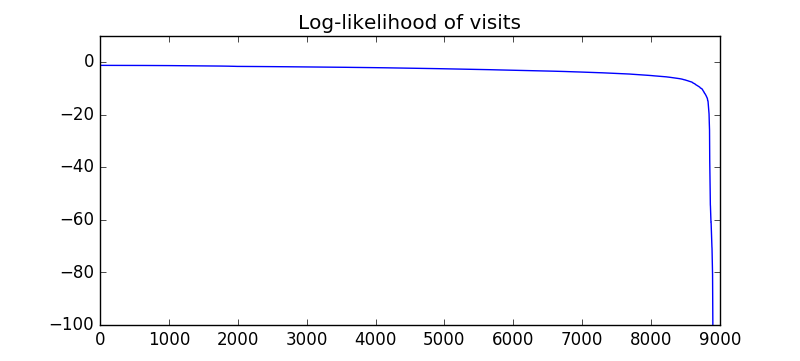
\includegraphics[width=\textwidth]{images/likelihood}
		\caption{Log-likelihood of all visits sorted in decreasing order.}
		\label{fig:likelihood}
	\end{center}
\end{figure}

\begin{figure}[!ht]
	\begin{center}
		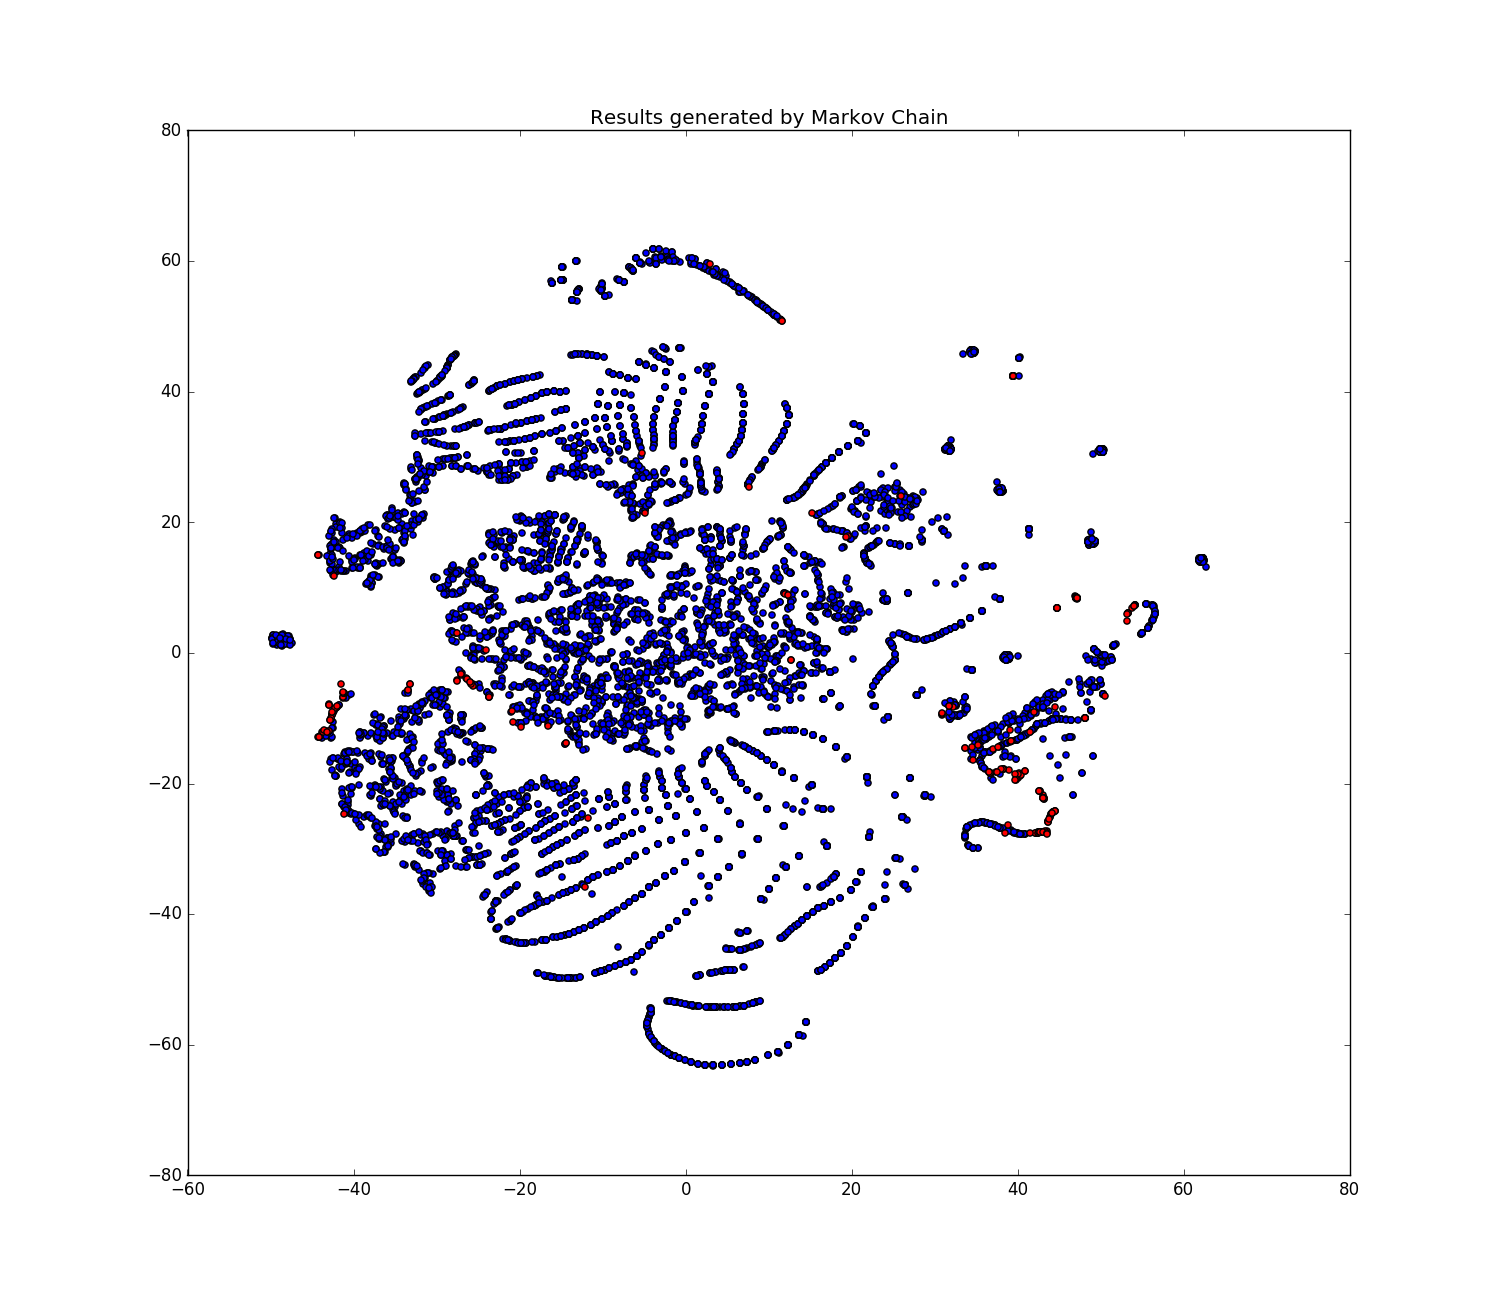
\includegraphics[width=\textwidth]{images/MarkovResult}
		\caption{Results generated by first-order Markov Chain using negative binomial distribution as emission function, visualized using t-SNE. Anomalies are painted in red.}
		\label{fig:MarkovResult}
	\end{center}
\end{figure}

\section{Discussion}
\label{sec:discuss}
Above result suggests both DBSCAN and Markov Chain can spot out anomalies. However, compared to DBSCAN, we think Markov Chain is a better method for several reasons. 

Firstly, clusters formed by DBSCAN are slightly contaminated. For example, the 4th visit in cluster 7 seems very abnormal and should appear in other clusters. Other clusters also have entries does not resemble other visits in this log. A reason for such behaviour is the hard assignment to clusters in DBSCAN. In Markov Chain, however, each visit is assigned by a score which indicates how ``normally'' this visit is. This ``soft-assignment'' is a better description of the entries. Besides, the user has to interpret the meaning of each cluster by themselves, which is typically unexpected by the user.

Secondly, Markov Chain has better time and space complexity for detecting future anomalies. When determine if a new visit log is anomaly, DBSCAN will compare this new visit to all past visits and then assign this new visit to the cluster fitting it best. Thus, DBSCAN requires to maintain all past visits, and new detection takes $O(n)$ time. This requirement will gradually becomes impractical. In contrast, Markov Chain only needs to maintain the computed parameters of transition matrix and emission functions. Computing the log-likelihood takes $O(1)$ time for each new visit log. Thus, speaking from this aspect, Markov Chain is a much better method than DBSCAN.
 
\chapter{Discussion}
\label{chapter:discussion}

At this point, you will have some insightful thoughts on your implementation
and you may have ideas on what could be done in the future. 
This chapter is a good place to discuss your thesis as a whole and to show your
professor that you have really understood some non-trivial aspects of the
methods you used\ldots


 
\chapter{Conclusions}
\label{chapter:conclusions}

Time to wrap it up! 
Write down the most important findings from your work. 
Like the introduction, this chapter is not very long.
Two to four pages might be a good limit. 



% Load the bibliographic references
% ------------------------------------------------------------------
% You can use several .bib files:
% \bibliography{thesis_sources,ietf_sources}
\bibliography{sources}


% Appendices go here
% ------------------------------------------------------------------
% If you do not have appendices, comment out the following lines
\appendix
\chapter{First appendix}
\label{chapter:Visit Samples}

{\scriptsize
\begin{longtable}{|c|p{0.9\textwidth}|}
\caption{10 samples from each cluster formed by DBSCAN}
\label{tab:samplesFromCluster}\\
		\hline
		Cluster No. & Samples \\
		\hline
		\multirow{10}{*}{Cluster 0}
		& 945438 ENROLLING 0 WAITING 77 WAITING -1 \\
		& 1230357 ENROLLING 45 WAITING 13 WAITING -1 \\
		& 1960464 ENROLLING 3 WAITING 24 WAITING -1 \\
		& 14813553 ENROLLING 8 WAITING 33 WAITING -1 \\
		& 15253762 ENROLLING 1 WAITING 70 WAITING -1 \\
		& 15254301 ENROLLING 110 WAITING -1 \\
		& 16146920 ENROLLING 128 WAITING 4 IN\_TREATMENT\_ROOM 52 CLOSED -1 \\
		& 16335930 ENROLLING 1 WAITING 16 WAITING 5 WAITING 1 CANCELLED -1 \\
		& 16759935 ENROLLING 33 WAITING 55 WAITING -1 \\
		& 16760057 ENROLLING 0 WAITING 0 IN\_TREATMENT\_ROOM 53 CANCELLED -1 \\
		\hline
		\multirow{10}{*}{Cluster 1}
		& 8490996 ENROLLING 0 WAITING 71 WAITING 0 WAITING -1 \\
		& 13585666 ENROLLING 0 WAITING 78 WAITING -1 \\
		& 15636771 ENROLLING 2 WAITING 23 WAITING -1 \\
		& 16760229 ENROLLING 0 WAITING 76 WAITING -1 \\
		& 17383819 ENROLLING 106 WAITING 0 WAITING -1 \\
		& 17383955 ENROLLING 0 WAITING 18 WAITING 0 WAITING -1 \\
		& 18441848 ENROLLING 222 WAITING 0 WAITING -1 \\
		& 20080659 ENROLLING 0 WAITING 30 WAITING 0 WAITING -1 \\
		& 20330934 ENROLLING 97 WAITING 0 WAITING -1 \\
		& 20454780 WAITING 1 WAITING 239 WAITING 0 WAITING 0 WAITING -1 \\
		\hline
		\multirow{10}{*}{Cluster 2}
		& 15253761 ENROLLING 1 WAITING 27 IN\_TREATMENT\_ROOM 43 CLOSED -1 \\
		& 15833795 ENROLLING 28 WAITING 48 IN\_TREATMENT\_ROOM 6 CLOSED -1 \\
		& 15845553 ENROLLING 0 WAITING 16 IN\_TREATMENT\_ROOM 9 CLOSED -1 \\
		& 15856901 ENROLLING 1 WAITING 4 IN\_TREATMENT\_ROOM 4 CLOSED -1 \\
		& 15982252 ENROLLING 3 WAITING 2 IN\_TREATMENT\_ROOM 12 CLOSED -1 \\
		& 16080179 ENROLLING 1 WAITING 3 IN\_TREATMENT\_ROOM 5 CLOSED -1 \\
		& 16239380 ENROLLING 1 WAITING 1 IN\_TREATMENT\_ROOM 10 CLOSED -1 \\
		& 16240164 ENROLLING 0 WAITING 41 IN\_TREATMENT\_ROOM 13 CLOSED -1 \\
		& 16261761 ENROLLING 0 WAITING 1 IN\_TREATMENT\_ROOM 21 CLOSED -1 \\
		& 16285157 ENROLLING 22 WAITING 16 IN\_TREATMENT\_ROOM 4 CLOSED -1 \\
		\hline
		\multirow{10}{*}{Cluster 3}
		& 16270356 ENROLLING 1 WAITING 124 WAITING -1 \\
		& 16718646 ENROLLING 1533 CANCELLED -1 \\
		& 16802740 ENROLLING 480 CANCELLED -1 \\
		& 16803188 ENROLLING 35 CANCELLED -1 \\
		& 16808873 ENROLLING 1533 CANCELLED -1 \\
		& 16820174 ENROLLING 173 CANCELLED -1 \\
		& 16847486 ENROLLING 3 CANCELLED -1 \\
		& 16848514 ENROLLING 91 CANCELLED -1 \\
		& 16896527 ENROLLING 84 CANCELLED -1 \\
		& 16911990 ENROLLING 100 CANCELLED -1 \\
		\hline
		\multirow{10}{*}{Cluster 4}
		& 16759931 ENROLLING 1 WAITING 0 IN\_TREATMENT\_ROOM 89 CLOSED -1 \\
		& 16759933 ENROLLING 12 WAITING 0 IN\_TREATMENT\_ROOM 35 CLOSED -1 \\
		& 16759945 ENROLLING 93 WAITING 0 IN\_TREATMENT\_ROOM 5 CLOSED -1 \\
		& 16760072 ENROLLING 33 WAITING 0 IN\_TREATMENT\_ROOM 5 CLOSED -1 \\
		& 16760633 ENROLLING 8 WAITING 0 IN\_TREATMENT\_ROOM 45 CLOSED -1 \\
		& 16760641 ENROLLING 24 WAITING 0 IN\_TREATMENT\_ROOM 2 CLOSED -1 \\
		& 16802066 ENROLLING 1 WAITING 0 IN\_TREATMENT\_ROOM 19 CLOSED -1 \\
		& 16802074 ENROLLING 3 WAITING 0 IN\_TREATMENT\_ROOM 5 CLOSED -1 \\
		& 16802391 ENROLLING 1 WAITING 0 IN\_TREATMENT\_ROOM 22 CLOSED -1 \\
		& 16802516 ENROLLING 2 WAITING 0 IN\_TREATMENT\_ROOM 23 CLOSED -1 \\
		\hline
		\multirow{10}{*}{Cluster 5}
		& 16760211 ENROLLING 0 WAITING 36 CANCELLED -1 \\
		& 16802397 ENROLLING 0 WAITING 58 CANCELLED -1 \\
		& 16802538 WAITING 49 CANCELLED -1 \\
		& 16802716 ENROLLING 0 WAITING 2 CANCELLED -1 \\
		& 16802724 ENROLLING 0 WAITING 9 CANCELLED -1 \\
		& 16803196 ENROLLING 0 WAITING 2 CANCELLED -1 \\
		& 16808893 ENROLLING 0 WAITING 0 WAITING 23 CANCELLED -1 \\
		& 16824757 WAITING 3 CANCELLED -1 \\
		& 16825742 WAITING 1 CANCELLED -1 \\
		& 16841048 ENROLLING 0 WAITING 0 WAITING 2 CANCELLED -1 \\
		\hline
		\multirow{10}{*}{Cluster 6}
		& 16760216 ENROLLING 27 WAITING 92 IN\_TREATMENT\_ROOM 0 CLOSED -1 \\
		& 16802089 ENROLLING 0 WAITING 92 IN\_TREATMENT\_ROOM 0 CLOSED -1 \\
		& 16803170 ENROLLING 0 WAITING 17 IN\_TREATMENT\_ROOM 0 CLOSED -1 \\
		& 16883234 WAITING 1 IN\_TREATMENT\_ROOM 0 CLOSED -1 \\
		& 16889884 ENROLLING 0 WAITING 6 IN\_TREATMENT\_ROOM 0 CLOSED -1 \\
		& 17137323 ENROLLING 2 WAITING 4 IN\_TREATMENT\_ROOM 0 CLOSED -1 \\
		& 17144229 ENROLLING 2 WAITING 66 IN\_TREATMENT\_ROOM 0 CLOSED -1 \\
		& 17266404 ENROLLING 34 WAITING 48 IN\_TREATMENT\_ROOM 0 CLOSED -1 \\
		& 17266727 ENROLLING 44 WAITING 21 IN\_TREATMENT\_ROOM 0 CLOSED -1 \\
		& 17383049 ENROLLING 0 WAITING 33 IN\_TREATMENT\_ROOM 0 CLOSED -1 \\
		\hline
		\multirow{10}{*}{Cluster 7}
		& 16760390 ENROLLING 0 WAITING 0 IN\_TREATMENT\_ROOM 13 CLOSED -1 \\
		& 16801915 ENROLLING 0 WAITING 0 IN\_TREATMENT\_ROOM 7 CLOSED -1 \\
		& 16802224 ENROLLING 0 WAITING 0 IN\_TREATMENT\_ROOM 8 CLOSED -1 \\
		& 16802368 ENROLLING 195 WAITING 37 IN\_TREATMENT\_ROOM 2 WAITING 2929 ENROLLING 0 WAITING 0 IN\_TREATMENT\_ROOM 21 CLOSED -1 \\
		& 16802390 ENROLLING 0 WAITING 0 IN\_TREATMENT\_ROOM 4 CLOSED -1 \\
		& 16802750 ENROLLING 0 WAITING 0 IN\_TREATMENT\_ROOM 7 CLOSED -1 \\
		& 16803047 ENROLLING 0 WAITING 0 IN\_TREATMENT\_ROOM 3 CLOSED -1 \\
		& 16803314 ENROLLING 0 WAITING 0 IN\_TREATMENT\_ROOM 8 CLOSED -1 \\
		& 16824756 ENROLLING 0 WAITING 0 IN\_TREATMENT\_ROOM 41 CLOSED -1 \\
		& 16824867 ENROLLING 0 WAITING 0 IN\_TREATMENT\_ROOM 10 CLOSED -1 \\
		\hline
		\multirow{10}{*}{Cluster 8}
		& 16825520 ENROLLING 72 WAITING 7 IN\_TREATMENT\_ROOM 39 CLOSED -1 \\
		& 16825742 ENROLLING 2 WAITING 0 CANCELLED -1 \\
		& 16847801 ENROLLING 53 WAITING 1 CANCELLED -1 \\
		& 16896665 ENROLLING 3 WAITING 8 WAITING 0 CANCELLED -1 \\
		& 16898355 ENROLLING 50 WAITING 1 CANCELLED -1 \\
		& 17149264 ENROLLING 11 WAITING 0 CANCELLED -1 \\
		& 17266883 ENROLLING 1 WAITING 55 WAITING 0 CANCELLED -1 \\
		& 17383018 ENROLLING 3 WAITING 113 IN\_TREATMENT\_ROOM 7 CLOSED -1 \\
		& 17383043 ENROLLING 9 WAITING 42 IN\_TREATMENT\_ROOM 73 CLOSED -1 \\
		& 17383842 ENROLLING 11 WAITING 1 CANCELLED -1 \\
		\hline
		\multirow{10}{*}{Cluster 9}
		& 16896538 ENROLLING 1 WAITING 32 CANCELLED -1 \\
		& 16898635 ENROLLING 1 WAITING 6 CANCELLED -1 \\
		& 17073845 ENROLLING 1 WAITING 5 IN\_TREATMENT\_ROOM 0 WAITING 6 IN\_TREATMENT\_ROOM 6 CLOSED -1 \\
		& 17137406 ENROLLING 44 WAITING 3 IN\_TREATMENT\_ROOM 56 CLOSED -1 \\
		& 17137437 ENROLLING 1 WAITING 56 CANCELLED -1 \\
		& 17137811 ENROLLING 1 WAITING 18 CANCELLED -1 \\
		& 17147824 ENROLLING 0 WAITING 1323 CANCELLED -1 \\
		& 17250342 ENROLLING 1 WAITING 68 CANCELLED -1 \\
		& 17383392 ENROLLING 42 WAITING 3 IN\_TREATMENT\_ROOM 50 CLOSED -1 \\
		& 17383812 ENROLLING 1 WAITING 7 CANCELLED -1 \\
		\hline
		\multirow{10}{*}{Cluster 10}
		& 16896542 WAITING 0 WAITING 4 WAITING -1 \\
		& 16898754 ENROLLING 10 WAITING 55 IN\_TREATMENT\_ROOM 2 CLOSED -1 \\
		& 16911970 WAITING 239 CANCELLED -1 \\
		& 18042974 ENROLLING 8 WAITING 1 IN\_TREATMENT\_ROOM 71 CLOSED -1 \\
		& 18206521 ENROLLING 0 WAITING 0 WAITING 136 CANCELLED -1 \\
		& 18206522 ENROLLING 0 WAITING 0 WAITING 136 CANCELLED -1 \\
		& 19336998 ENROLLING 0 WAITING 1 IN\_TREATMENT\_ROOM 21 WAITING 0 WAITING 536 CANCELLED -1 \\
		& 19488319 WAITING 13 WAITING 0 WAITING 0 CANCELLED -1 \\
		& 19517799 WAITING 215 CANCELLED -1 \\
		& 19551936 ENROLLING 3 WAITING 0 WAITING 154 CANCELLED -1 \\
		\hline
		\multirow{10}{*}{Cluster 11}
		& 17141316 ENROLLING 3 WAITING 24 CANCELLED -1 \\
		& 17267028 ENROLLING 59 WAITING 13 IN\_TREATMENT\_ROOM 69 CLOSED -1 \\
		& 17333621 ENROLLING 1 WAITING 1 CANCELLED -1 \\
		& 17384117 ENROLLING 40 WAITING 11 IN\_TREATMENT\_ROOM 52 CLOSED -1 \\
		& 17384134 ENROLLING 1 WAITING 105 IN\_TREATMENT\_ROOM 92 CLOSED -1 \\
		& 17445733 ENROLLING 1104 ENROLLING -1 \\
		& 17472038 ENROLLING 9 WAITING 37 IN\_TREATMENT\_ROOM 70 CLOSED -1 \\
		& 17472501 ENROLLING 52 WAITING 118 IN\_TREATMENT\_ROOM 22 CLOSED -1 \\
		& 17484544 ENROLLING 0 WAITING 1457 ENROLLING 0 WAITING -1 \\
		& 17512538 ENROLLING 0 WAITING 16 WAITING 1002 CANCELLED -1 \\
		\hline
\end{longtable}
}

\newpage
{\scriptsize
\begin{longtable}{|c|p{0.9\textwidth}|}
\caption{Samples with log-likelihood computed using first-order Markov Chain using negative binomial distribution as emission function.}
\label{tab:samplesFromGenerative}\\
\hline
log-likelihood & sample \\ \hline
-1.22501248649 & 21332189 ENROLLING 0 WAITING 3 IN\_TREATMENT\_ROOM 5 CLOSED -1 \\
-1.22501248649 & 21332152 ENROLLING 0 WAITING 3 IN\_TREATMENT\_ROOM 5 CLOSED -1 \\
-1.22501248649 & 21243121 ENROLLING 0 WAITING 3 IN\_TREATMENT\_ROOM 5 CLOSED -1 \\
-1.22501248649 & 21242603 ENROLLING 0 WAITING 3 IN\_TREATMENT\_ROOM 5 CLOSED -1 \\
-1.22501248649 & 20753590 ENROLLING 0 WAITING 3 IN\_TREATMENT\_ROOM 5 CLOSED -1 \\
\hline
-1.31252682278 & 20531975 ENROLLING 0 WAITING 9 IN\_TREATMENT\_ROOM 5 CLOSED -1 \\
-1.31252682278 & 20335903 ENROLLING 0 WAITING 9 IN\_TREATMENT\_ROOM 5 CLOSED -1 \\
-1.31252682278 & 20332176 ENROLLING 0 WAITING 9 IN\_TREATMENT\_ROOM 5 CLOSED -1 \\
-1.31252682278 & 20330946 ENROLLING 0 WAITING 9 IN\_TREATMENT\_ROOM 5 CLOSED -1 \\
-1.31252682278 & 19524600 ENROLLING 0 WAITING 9 IN\_TREATMENT\_ROOM 5 CLOSED -1 \\
-1.31252682278 & 18895611 ENROLLING 0 WAITING 9 IN\_TREATMENT\_ROOM 5 CLOSED -1 \\
\hline
-1.6200398225 & 20090272 ENROLLING 0 WAITING 20 IN\_TREATMENT\_ROOM 5 CLOSED -1 \\
-1.6200398225 & 17137238 ENROLLING 0 WAITING 20 IN\_TREATMENT\_ROOM 5 CLOSED -1 \\
-1.6200398225 & 17137111 ENROLLING 0 WAITING 20 IN\_TREATMENT\_ROOM 5 CLOSED -1 \\
-1.6200398225 & 16803024 ENROLLING 0 WAITING 20 IN\_TREATMENT\_ROOM 5 CLOSED -1 \\
-1.62051607252 & 21419996 ENROLLING 0 WAITING 14 IN\_TREATMENT\_ROOM 13 CLOSED -1 \\
\hline
-1.81955956629 & 18946307 ENROLLING 1 WAITING 0 IN\_TREATMENT\_ROOM 10 CLOSED -1 \\
-1.81955956629 & 17010037 ENROLLING 1 WAITING 0 IN\_TREATMENT\_ROOM 10 CLOSED -1 \\
-1.81974417979 & 20538959 ENROLLING 1 WAITING 5 IN\_TREATMENT\_ROOM 13 CLOSED -1 \\
-1.81974417979 & 16824641 ENROLLING 1 WAITING 5 IN\_TREATMENT\_ROOM 13 CLOSED -1 \\
-1.82019772133 & 19969197 ENROLLING 2 WAITING 7 IN\_TREATMENT\_ROOM 6 CLOSED -1 \\
\hline
-2.09969260165 & 21332560 ENROLLING 6 WAITING 4 IN\_TREATMENT\_ROOM 8 CLOSED -1 \\
-2.09974363796 & 21419663 ENROLLING 1 WAITING 1 IN\_TREATMENT\_ROOM 19 CLOSED -1 \\
-2.10057254235 & 19664612 ENROLLING 1 WAITING 19 IN\_TREATMENT\_ROOM 11 CLOSED -1 \\
-2.10063359561 & 17267455 ENROLLING 3 WAITING 9 IN\_TREATMENT\_ROOM 12 CLOSED -1 \\
-2.10077419383 & 20538310 ENROLLING 1 WAITING 20 IN\_TREATMENT\_ROOM 10 CLOSED -1 \\
\hline
-2.52467325597 & 18335666 ENROLLING 1 WAITING 33 IN\_TREATMENT\_ROOM 10 CLOSED -1 \\
-2.52507176943 & 18243950 ENROLLING 1 WAITING 35 IN\_TREATMENT\_ROOM 4 CLOSED -1 \\
-2.52507176943 & 16911955 ENROLLING 1 WAITING 35 IN\_TREATMENT\_ROOM 4 CLOSED -1 \\
-2.52523586276 & 18160697 ENROLLING 2 WAITING 31 IN\_TREATMENT\_ROOM 5 CLOSED -1 \\
-2.52574525145 & 19841457 ENROLLING 7 WAITING 20 IN\_TREATMENT\_ROOM 7 CLOSED -1 \\
\hline
-3.06107298199 & 19954450 ENROLLING 0 WAITING 61 IN\_TREATMENT\_ROOM 3 CLOSED -1 \\
-3.06260151935 & 21127113 ENROLLING 11 WAITING 30 IN\_TREATMENT\_ROOM 9 CLOSED -1 \\
-3.06387434043 & 19230307 ENROLLING 28 WAITING 10 IN\_TREATMENT\_ROOM 11 CLOSED -1 \\
-3.06458227144 & 18247745 ENROLLING 2 WAITING 10 IN\_TREATMENT\_ROOM 33 CLOSED -1 \\
-3.06629701355 & 17141536 ENROLLING 26 WAITING 13 IN\_TREATMENT\_ROOM 2 CLOSED -1 \\
\hline
-3.77652544852 & 20624690 ENROLLING 7 WAITING 54 IN\_TREATMENT\_ROOM 11 CLOSED -1 \\
-3.77716200844 & 19230163 ENROLLING 0 WAITING 32 IN\_TREATMENT\_ROOM 43 CLOSED -1 \\
-3.77716858350 & 17266875 ENROLLING 3 WAITING 25 IN\_TREATMENT\_ROOM 36 CLOSED -1 \\
-3.77756155251 & 16848287 ENROLLING 58 WAITING 10 IN\_TREATMENT\_ROOM 8 CLOSED -1 \\
-3.77963738529 & 17384149 ENROLLING 1 WAITING 42 CANCELLED -1 \\
\hline
-5.10571464997 & 20032830 ENROLLING 28 CANCELLED -1 \\
-5.10571464997 & 18004184 ENROLLING 28 CANCELLED -1 \\
-5.10571464997 & 18004183 ENROLLING 28 CANCELLED -1 \\
-5.10766253514 & 18945732 ENROLLING 30 WAITING 11 IN\_TREATMENT\_ROOM 48 CLOSED -1 \\
-5.10842170221 & 18043295 ENROLLING 0 WAITING 19 IN\_TREATMENT\_ROOM 71 CLOSED -1 \\
-5.11050052549 & 20538023 ENROLLING 60 WAITING 8 CANCELLED -1 \\
\hline
-227.515556821 & 18883776 ENROLLING 0 WAITING 4435 ENROLLING -1 \\
-294.647987389 & 19593547 ENROLLING 0 WAITING 5754 ENROLLING -1 \\
-653.392679598 & 19229957 ENROLLING 37265 ENROLLING 40 WAITING 1 IN\_TREATMENT\_ROOM 4 CLOSED -1 \\
-876.235768456 & 21127118 ENROLLING 50174 ENROLLING 0 WAITING 1 IN\_TREATMENT\_ROOM 3 CLOSED -1 \\
-1227.10081314 & 17144893 ENROLLING 0 WAITING 23 WAITING 48064 ENROLLING 0 WAITING 18 CANCELLED -1 \\
\hline

\end{longtable}
}


% End of document!
% ------------------------------------------------------------------
% The LastPage package automatically places a label on the last page.
% That works better than placing a label here manually, because the
% label might not go to the actual last page, if LaTeX needs to place
% floats (that is, figures, tables, and such) to the end of the 
% document.
\end{document}
